\documentclass[
	12pt,
	a4paper,
	ngerman,
	%twoside,
	BCOR=8mm,
	headings=normal,
	parskip=half,
	headsepline,
	automark,
	listof=totoc,
	bibliography=totoc,
	%,captions=tableabove
	%draft
]{scrreprt}
%
%
%%%%%%%%%%%%%%%%%%%%%%%%%%%%%%%%%%%%%%%%%%%%%%%%%%%%%%%%%%%%%%%%%%%%%%%%%%%%%%%
% Pakete laden
%%%%%%%%%%%%%%%%%%%%%%%%%%%%%%%%%%%%%%%%%%%%%%%%%%%%%%%%%%%%%%%%%%%%%%%%%%%%%%%
%
\usepackage{ifluatex}
\usepackage{babel}
%
\ifluatex
 % LuaLaTeX
 \usepackage{fontspec}
 \usepackage{selnolig}
\else
 % PdfLaTeX
 \usepackage[T1]{fontenc}
\fi
%
\usepackage{csquotes}
\usepackage{scrlayer-scrpage}
\usepackage{microtype}
%
%\usepackage{ziffer}% optional
%\usepackage[locale=DE]{siunitx}% optional
%
\usepackage{tikz}
\usepackage{pgfplots}
%
\usepackage[backend=biber]{biblatex}
%
\usepackage{amsmath}
\usepackage{amssymb}
%
\usepackage{hyperref}
%
%=== wichtig, dass folgende Pakete NACH hyperref geladen werden ===============
\usepackage{scrhack}% Um Warnung bzgl. \float@addtolists im listings-Paket (s.u.) zu vermeiden
\usepackage{listings}
%
\usepackage[nameinlink]{cleveref}
\usepackage[all]{hypcap}
\usepackage[
	toc,
	symbols,
	acronyms,
]{glossaries}
%%%%%%%%%%%%%%%%%%%%%%%%%%%%%%%%%%%%%%%%%%%%%%%%%%%%%%%%%%%%%%%%%%%%%%%%%%%%%%%
% Globale Definitionen
%%%%%%%%%%%%%%%%%%%%%%%%%%%%%%%%%%%%%%%%%%%%%%%%%%%%%%%%%%%%%%%%%%%%%%%%%%%%%%%


%=== pdf Metadaten ============================================================
\hypersetup{
	pdfauthor={Jurek Miklas Jesse},
	pdftitle={Implementierung eines Dashboard für Pentesting in einer Digital Forensik and Incident Response (DFIR) Umgebung für Open RAN},
	pdfsubject={Abschlussarbeit},
	pdfkeywords={
		Abschlussarbeit,
		DFIR,
		OPENRAN,
		ORAN,
		5G
	},
	bookmarksnumbered=true,
	pdfstartview=FitH,
	hidelinks,
}

%=== Kopf-/Fusszeile definieren ===============================================
\clearpairofpagestyles
\ohead[]{\headmark}
\ofoot[\pagemark]{\pagemark}

%=== Farben definieren ========================================================
\definecolor{THRed}{RGB}{207,24,32}
\definecolor{THOrange}{RGB}{236,101,37}
\definecolor{THPurple}{RGB}{175,54,140}

%=== Einstellungen für cref ===================================================
\newcommand{\crefpairconjunction}{ und~}
\newcommand{\crefrangeconjunction}{ bis~}
\crefname{figure}{Abbildung}{Abbildungen}
% Define custom colors
\definecolor{mygray}{rgb}{0.95,0.95,0.95}

% Define a custom environment for code blocks
\lstnewenvironment{code}[1][] % Optional argument for customization
{
  \lstset{
    backgroundcolor=\color{mygray},
    basicstyle=\ttfamily\scriptsize,
    breaklines=true,
    breakatwhitespace=true,
    frame=single,
    rulecolor=\color{gray},
    xleftmargin=5mm,
    numbers=left,
    numberstyle=\tiny,
    captionpos=b, % Position of the caption (b for bottom, t for top)
	float, % Hinzufügen der float-Option
    floatplacement=H,
    #1 % Allow overriding settings using optional arguments
  }
}
{}

%=== Einstellungen für plots ==================================================
\pgfplotsset{
	compat=newest,
	/pgf/number format/.cd,
	dec sep={\text{,}},
	1000 sep={\,},
}

%=== Einstellungen für listings ===============================================
\lstdefinestyle{myLaTeX}{
	basicstyle=\footnotesize\ttfamily,
	language=TeX,
	keywordstyle=\color{blue},
	frame=single,
	backgroundcolor=\color{gray!10},
	tabsize=2,
	morekeywords={
		lstdefinestyle,
		footnotesize,
		ttfamily,
		color,
	},
}

\lstdefinestyle{myBasic}{
	basicstyle=\footnotesize\ttfamily,
	frame=single,
	escapechar={|_},
	backgroundcolor=\color{white},
	keywordstyle=\color{black},
}

\lstset{style=myLaTeX}

\newcommand{\oran}{O-RAN}
\newcommand{\orana}{O-RAN Alliance}
%%%%%%%%%%%%%%%%%%%%%%%%%%%%%%%%%%%%%%%%%%%%%%%%%%%%%%%%%%%%%%%%%%%%%%%%%%%%%%%
% Begriffe für Glossar definieren
%%%%%%%%%%%%%%%%%%%%%%%%%%%%%%%%%%%%%%%%%%%%%%%%%%%%%%%%%%%%%%%%%%%%%%%%%%%%%%%

%=== Abkürzungen ==============================================================
\newacronym{foran}{5G-FORAN}{IT-Forensik und Behandlung von IT-Sicherheitsvorfällen im Open RAN}
\newacronym{acema}{ACEMA}{A Comprehensive Empirical Method to Analyze Threats in O-RAN Environments}
\newacronym{dfir}{DFIR}{Digital Forensics und Incident Response}
\newacronym[plural=Open RANs]{open-ran}{Open RAN}{Open Radio Access Network}
\newacronym{cvss}{CVSS}{Common Vulnerability Scoring System}
\newacronym{attack}{ATT\&CK}{Adversarial Tactics, Techniques, and Common Knowledge}
\newacronym[plural=CVEs]{cve}{CVE}{Common Vulnerabilities and Exposures}
\newacronym{bsi}{BSI}{Bundesamt für Sicherheit in der Informationstechnik}
\newacronym{wg11}{WG11}{Security Work Group}
\newacronym{wg1}{WG1}{Use Cases and Overall Architecture Group}
\newacronym{mitre}{MITRE}{MITRE Corporation}
\newacronym[plural=CWEs]{cwe}{CWE}{Common Weakness Enumeration}
\newacronym[plural=CAPECs]{capec}{CAPEC}{Common Attack Pattern Enumeration and Classification}
\newacronym{nis}{NIS}{Network and Information Systems Cooperation Group}
\newacronym{enisa}{ENISA}{The European Union Agency for Cybersecurity}
\newacronym{cli}{CLI}{Command Line Interface}
\newacronym{dnlab}{DN.Lab}{Labor für Datennetze}
\newacronym{vm}{VM}{virtuelle Maschine}
\newacronym{vscode}{VS Code}{Visual Studio Code}
\newacronym{ssh}{SSH}{Secure Shell Protocol}
\newacronym{tm4k}{TM4K}{Threat Matrix for Kubernetes}
\newacronym{cti}{CTI}{Cyber Threat Intelligence}
\newacronym{stix}{STIX}{Structured Threat Information Expression}
\newacronym{nist}{NIST}{National Institute of Standards and Technology}
\newacronym{nvd}{NVD}{National Vulnerability Database}
\newacronym{worm}{WORM}{Write-Once, Read-Many}
\newacronym{html}{HTML}{Hypertext Markup Language}
\newacronym{js}{JS}{JavaScript}
\newacronym{sc}{SC}{Software Community}
\newacronym[plural=RANs]{ran}{RAN}{Radio Access Network}
\newacronym[plural=RICs]{ric}{RIC}{RAN Intelligent Controller}
\newacronym{ktm}{KTM}{Kubernetes Threat Matrix}
\newacronym{hotwire}{Hotwire}{HTML-over-the-wire}
\newacronym{css}{CSS}{Cascading Style Sheets}
\newacronym{atlas}{ATLAS}{Adversarial Threat Landscape for Artificial-Intelligence Systems}
\newacronym[plural=ATs]{at}{AT}{ATTACK-Tool}
\newacronym{dot}{DOT}{Directed acyclic graph of tommorow}
\newacronym{o-du}{O-DU}{O-RAN Radio Unit}
\newacronym{o-cu}{O-RU}{O-RAN Central Unit}
%=== Symbole ==================================================================
% DELETE ME
\newglossaryentry{sym:force}{
	name=\ensuremath{\vec{F}},
	description={Kraft, vektorielle Größe},
	type=symbols,
}

%
\makeglossaries
%
\graphicspath{{images/}}
%
\addbibresource{references.bib}


\nocite{} % listet alle zitierten Quellen
%
\includeonly{
	content/0Cover,
	content/1chapAbstract,
	content/2chapKurzfassung,
	content/3chapEinleitung,
	content/4chapForschungsstand,
	content/5chapTechnischerHintergrund,
	content/6chapMethodik,
	content/7chapImplementierung,
	content/8chapDiskussion,
	content/9chapZusammenfassung,
	content/10chapDeclaration,
	anhang
}
%
%
%==============================================================================
%
\begin{document}
%
\pdfbookmark[0]{Titelseite}{titel}
\begin{titlepage}
    %
    %\sffamily% Umschalten auf serifenlose Schrift
    %
    \begin{center}
        % Define a minipage for each image to control width and alignment
        \begin{minipage}[c]{0.33\textwidth}
            
\includegraphics[height=2cm]{images/th_koeln.png} % Adjust height as needed
        \end{minipage}%
        \hfill
        \begin{minipage}[c]{0.1\textwidth}
            % Add an empty minipage in the center if necessary for spacing
        \end{minipage}%
        \hfill
        \begin{minipage}[c]{0.49\textwidth}
            \raisebox{0.1cm}{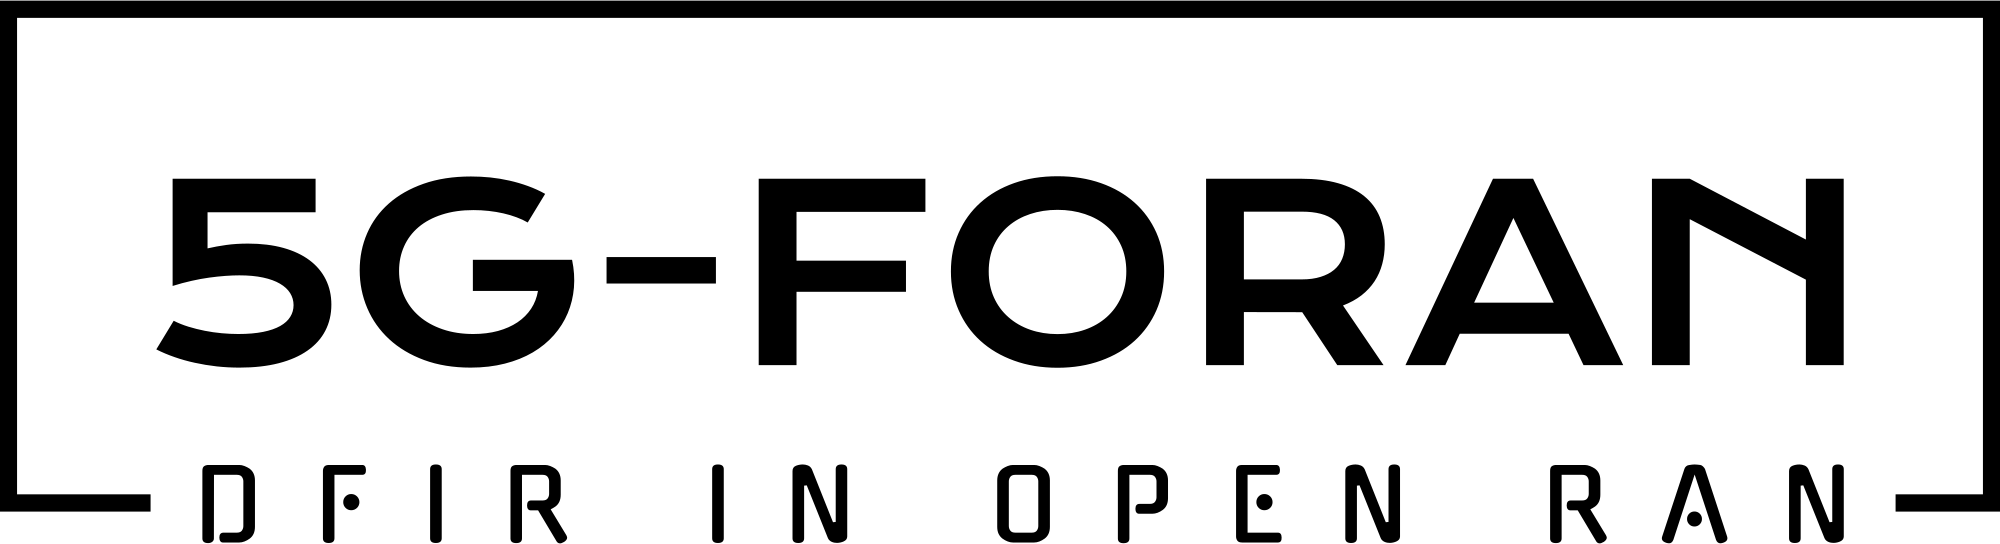
\includegraphics[height=2cm]{images/foran.png}} % Raise by 0.1cm
        \end{minipage}
        % Draw colored line below images
        \begin{tikzpicture}
            \fill[THRed] (0, 0) rectangle (\textwidth/3, 3pt);
            \fill[THOrange] (\textwidth/3, 0) rectangle (2*\textwidth/3, 3pt);
            \fill[THPurple] (2*\textwidth/3, 0) rectangle (\textwidth, 3pt);
        \end{tikzpicture}
    \end{center}
    %
    \vfill
    %
    \begin{center}
        \huge Implementierung eines Dashboard für Pentesting in einer Digital Forensics und Incident Response (DFIR) Umgebung für Open RAN\\[10mm]
    \end{center}
    %
    Bachelorarbeit zur Erlangung des akademischen Grades\newline
    \emph{Bachelor of Science}\newline
    im Studiengang Technische Informatik\newline
    an der Fakultät für Informations-, Medien- und Elektrotechnik\newline
    der Technischen Hochschule Köln
    %
    \vfill
    %
    \begin{tabular}{@{}ll}
        vorgelegt von:  & Jurek Miklas Jesse       \\
        Matrikel-Nr.:   & 11135480                 \\
        \\
        \\
        \\
        Erstgutachter:  & Prof. Dr. Andreas Grebe  \\
        Zweitgutachter: & Henrik Wittemeier, B.Sc.
    \end{tabular}
    %
    \vfill
    %
    Wiesbaden, TT.12.2024%
    %
    \rmfamily% Umschalten auf Standard-Schrift mit Serifen
    %
\end{titlepage}
\cleardoublepage
\pagenumbering{Roman}
\chapter*{Abstract}
\label{chap:abstract}
The dashboard developed in this work was specifically designed for use in \gls{dfir} environments for \gls{open-ran}, supporting penetration testing scenarios and enabling precise vulnerability assessments. The integration of the empirical \gls{acema} method and the use of \gls{cvss} data facilitate detailed analyses and visualizations. The dashboard provides a tool for visualizing and analyzing vulnerabilities in the highly virtualized Open RAN environment. Empirical evidence demonstrates which attack techniques pose significant risks or offer higher potential from an attacker{’}s perspective. The same findings were achieved in relation to O-RAN, where empirical and statistical methods identified components vulnerable to specific techniques. This work makes a significant contribution to security research while offering practical approaches for future developments and investigations in \gls{dfir} contexts.
\par Keywords: Open RAN, O-RAN, DFIR, 5G, Dashboard
\chapter*{Kurzfassung}
\label{chap:kurzfassung}
\glsreset{dfir}
\glsreset{open-ran}
Ein in dieser Arbeit entwickeltes Dashboard wurde speziell für den Einsatz in \gls{dfir}-Umgebungen für \gls{open-ran} entworfen, um Pentesting-Szenarien zu unterstützen und Schwachstellen präzise zu bewerten. Die Integration einer empirischen Methode und die Nutzung von CVSS-Daten ermöglichen detaillierte Analysen und Visualisierungen. Das Dashboard bietet ein Werkzeug zur Visualisierung und Analyse von Schwachstellen im stark virtualisierten Open RAN Umfeld. Es wird empirisch aufgezeigt, welche Angriffstechniken besonders risikobehaftet sind, beziehungsweise aus der Perspektive eines Angreifers ein höheres Potenzial bieten. Dasselbe Ergebnis wurde auch in Bezug auf O-RAN erreicht. Über empirische und statistische Methoden werden O-RAN Komponenten identifiziert, die bei Ausnutzung von spezifischen Techniken gefährdet sind. Es stellt einen wichtigen Beitrag zur Sicherheitsforschung dar und bietet zugleich Ansätze für zukünftige Entwicklungen und Untersuchungen in \gls{dfir}-Kontexten.
\par Schlüsselwörter: Open RAN, O-RAN, DFIR, 5G, Dashboard


\cleardoublepage
%
\pdfbookmark[0]{Inhaltsverzeichnis}{toc}
\tableofcontents
%
\listoftables
\listoffigures
\lstlistoflistings %Quelltextverzeichnis
%
\printglossary
\printglossary[type=\acronymtype, title={Abkürzungsverzeichnis}]
\printglossary[type=symbols, title={Symbolverzeichnis}]
%
\cleardoublepage
\KOMAoptions{open=right}
\pagenumbering{arabic}
\chapter{Einleitung}
\label{chap:Einleitung}

\par
Die Einführung des 5G-Netzwerks stellt einen bedeutenden Schritt in der Telekommunikationslandschaft dar und eröffnet durch die erhöhte Flexibilität und Geschwindigkeit neue Anwendungsfelder. Eine zentrale Entwicklung hierbei ist das Konzept von \gls{open-ran}, welches durch die offene Spezifikation und modulare Architektur das herkömmliche \gls{ran}-Design revolutioniert. \gls{open-ran} ermöglicht eine Interoperabilität zwischen verschiedenen Herstellern und eine flexiblere Verwaltung der Netzwerkkomponenten, was den Netzwerkbetreibern potenzielle Kosteneinsparungen und eine größere Anpassungsfähigkeit bietet. Die Abhängigkeit von proprietären Herstellen wie Huawei, Ericsson und Nokia fallen dabei weg \autocite{kimGeopoliticsNextGeneration2023}. Die \orana{}, ein Konsortium aus Telekommunikationsanbietern, Herstellern und Forschungsinstitutionen, treibt diesen Ansatz voran und entwickelt Standards und Architekturen, die speziell für 5G und zukünftig auch für 6G ausgelegt sind. Diese Standards sind auf die Entkopplung von Hardware und Software ausgelegt und fördern die Virtualisierung von RAN-Komponenten, um so die Flexibilität der Netzbetreiber zu erhöhen \autocite{o-ranallianceORANWhitePaper2018102018}.
\par
Das Forschungsprojekt \gls{foran}, eine Kooperation zwischen der Technischen Hochschule Köln und PROCYDE GmbH, widmet sich den sicherheitstechnischen Herausforderungen im O-RAN Umfeld, insbesondere im Kontext der \gls{dfir}. Ziel des Projekts ist die Entwicklung von Methoden zur Analyse, Behandlung und Behebung von Sicherheitsvorfällen in \gls{open-ran}-Netzwerken. Hierbei wird der gesamte Lebenszyklus eines Sicherheitsvorfalls berücksichtigt: von der Erkennung über die Analyse bis hin zur forensischen Nachverfolgung.
\par Das Projekt liefert wissenschaftliche Erkenntnisse zur Sicherheit von \gls{open-ran}-Systemen, indem neue Ansätze zur Analyse und Behandlung von Sicherheitsvorfällen entwickelt oder auf existierender Forschung aufgebaut wird. Die Verknüpfung empirischer Daten mit bewährten Sicherheitsmodellen wie dem \gls{mitre} \gls{attack}-Framework schafft eine wissenschaftliche Basis zur Bewertung von Risiken. Die Forschung trägt dazu bei, das Verständnis für die Bedrohungslandschaft in virtualisierten Mobilfunknetzen zu vertiefen und liefert Ansätze für die Weiterentwicklung von sicheren Implementierungen der O-RAN-Spezifikationen. Der wissenschaftliche Wert des Projekts liegt insbesondere in der Übertragbarkeit der entwickelten Methoden auf andere virtualisierte oder containerisierte Systeme sowie der Schaffung einer Grundlage für weiterführende Arbeiten im Bereich 5G- und 6G-Sicherheit.
\par Das Forschungsprojekt \gls{foran} ist in zwei Teilprojekte unterteilt: \gls{foran}-ATTACK und \gls{foran}-\gls{dfir}. Im Rahmen von \gls{foran}-ATTACK wird ein System entwickelt, das gezielte Angriffssimulationen auf \gls{open-ran}-Komponenten ermöglicht, um spezifische Angriffsspuren zu generieren. Diese Angriffsspuren können dann mit - im Teilprojekt \gls{foran}-\gls{dfir} - entwickelten Methoden identifiziert und behandelt werden. Dabei liegt der Fokus auf der Anpassung etablierter \gls{dfir}-Frameworks für die spezifischen Anforderungen im \gls{open-ran}-Bereich \autocite{5GFORAN}. Eine sehr wichtige Rolle bei der Kategorisierung von Angriffen und der Bewertung von Schwachstellen spielt die Arbeit des \gls{mitre}. Die \gls{mitre}-Corporation stellt unter anderem mit dem \gls{attack}-Framework eine umfassende strukturierte Sammlung von Angriffstechniken und -taktiken bereit \autocite{SolvingProblemsSafer2024,MITREATTCK}.
\par
In dieser Arbeit liegt der Fokus auf der Weiterentwicklung und Weiterimplementierung eines Dashboards, welches als zentrales Tool für die Visualisierung und Analyse von Angriffssimulationen fungiert. Das Dashboard stellt eine Komponente im ATTACK-Teilvorhaben von \gls{foran} dar. Zu den spezifischen Anforderungen zählen die Darstellung von Angriffspfaden und die Integration des \gls{cvss} zur Bedrohungsbewertung. Außerdem wurde speziell für die Kategorisierung der Angriffe eine abgewandelte Version der \gls{mitre} \gls{attack}-Matrix erstellt und die Daten empirisch eingeordnet. Dies unterstützt eine analytische Herangehensweise an die Bewertung der Angriffe \gls{open-ran} \autocite{dieterichDevelopmentAdversarySimulation2024}.
\par
Diese Arbeit implementiert die Methode, die \citeauthor{klementSecuring6GTransition2024} in ihrem Paper \textit{Toward Securing the 6G Transition: A Comprehensive Empirical Method to  Analyze Threats in O-RAN Environments}\footnote{Von den Autoren abgekürzt als ACEMA O-RAN, im Folgenden nur ACEMA} beschreiben, um Schwachstellen in \gls{open-ran}-Komponenten anhand empirischer Daten zu bewerten. Es wird hierbei keine Bewertung aller möglichen Angriffe vorgenommen, sondern die durch das Teilvorhaben \gls{foran}-ATTACK gefundenen und durch das \gls{at} simulierten Angriffe auf eine Referenzimplementierung von \gls{open-ran} der O-RAN Software Community bewertet. Die Bewertung nach dem \gls{cvss} wird in der Übersicht einzelner Angriffe und in der modifizierten \gls{mitre}-Matrix dargestellt \autocite{dieterichDevelopmentAdversarySimulation2024,klementSecuring6GTransition2024}.
\todo{Worum es in der Arbeit wirklich geht steht nur im letzten Absatz. Vielleicht da noch ein bisschen mehr drüber schreiben. }

\chapter{Stand der Wissenschaft}
\label{chap:forschungsstand}
Seit den Anfängen der Entwicklung von \gls{open-ran} im Februar 2016 und der Gründung der \orana{} 2018 gibt es einige\todo{Hier anderes Wort?} wissenschaftliche Arbeiten, die sich mit dem Thema Schwachstellenanalyse und Schwachstellenbewertung in einer \gls{open-ran} Umgebung beschäftigen \autocite{ORANAlliance,GuideOpenRAN}. Unter dem Stichwort \glqq{}O-RAN\grqq{} finden sich über die \gls{mitre} \gls{cve} Suche aktuell 12 Einträge, die Schwachstellen in der O-RAN-SC-Referenzimplementierung betreffen \autocite{CVESearchResults}. Die systematische Suche nach und Analyse von Schwachstellen ist entscheidend, um Sicherheitslücken frühzeitig zu erkennen und geeignete Gegenmaßnahmen zu implementieren. In diesem Kapitel wird ein Überblick über den Forschungsstand anhand einer Auswahl von Arbeiten gegeben.

%
\section{Technischer Report der O-RAN Alliance Security Work Group}
\label{sec:forschungsstand-wg11}
Die \gls{wg11} der \orana{} beschäftigt sich mit den sicherheitstechnischen Aspekten von \gls{open-ran} und veröffentlicht in regelmäßigen Abständen einen technischen Report, der eine Bedrohungsmodellierung und Risikobeurteilung enthält. Zum Zeitpunkt der Veröffentlichung ist der Report in Version \textit{\textsf{v04.00}} die neueste Fassung dieses Dokuments. Der Report umfasst sowohl mögliche O-RAN-spezifische Angriffe auf Komponenten und Schnittstellen in einem \gls{open-ran}-System, als auch nicht O-RAN-spezifische Bedrohungen, wie Supply-Chain-Angriffe auf Quell-Offenen Programmcode oder physischen Eingriff um Zugriff auf sensible Daten zu erlangen, die in allen \glspl{open-ran} existieren können \autocite{o-ranworkgroup11securityworkgroupORANSecurityThreat2024}. Im Folgenden wird ein Überblick über die O-RAN-spezifischen Bedrohungen gegeben. Die davon betroffenen Komponenten und Schnittstellen sind in Abbildung \ref{fig:oran-architecture} dargestellt.
\begin{figure}
    \centering
    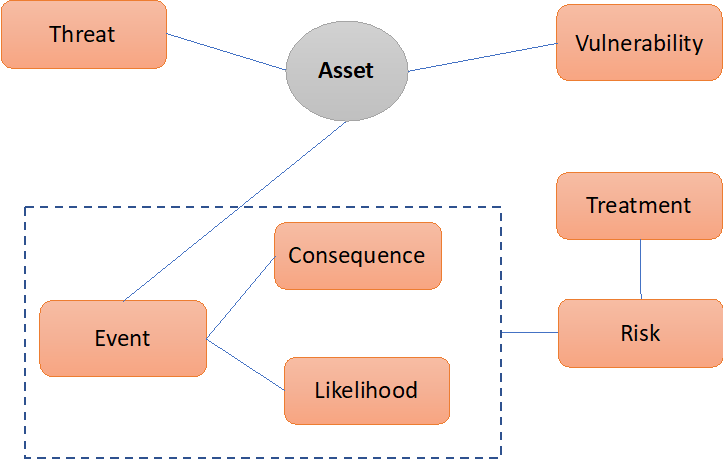
\includegraphics[width=0.5\textwidth]{oran-risk-factors}
    \caption{Einflussfaktoren für die Risikobeurteilung (Quelle: \autocite{o-ranworkgroup11securityworkgroupORANSecurityThreat2024})}
    \label{fig:oran-risk-factors}
\end{figure}
\par Es wird betrachtet wie hoch die Wahrscheinlich (\textit{Likelihood}) ist, dass eine Schwachstelle (\textit{Vulnerability}) durch eine spezifische Bedrohung (\textit{Threat}) ausgenutzt wird, und welche Konsequenzen (\textit{Consequences}) dies für das Asset hat. Die \orana{} definiert als Basis für die Risikobewertung eine Reihe von Einflussfaktoren, die in Abbildung \ref{fig:oran-risk-factors} dargestellt sind. Ein Asset ist dabei eine (Teil-)Komponente oder eine Schnittstelle zwischen Komponenten. Die \gls{wg11} identifiziert dazu 35 Bedrohungen in der Komponente \textit{O-RAN Cloud} und 69 Bedrohungen die auf alle anderen Komponenten und Schnittstellen zutreffen \autocite{o-ranworkgroup11securityworkgroupORANSecurityThreat2024}. Die \orana{} definiert in ihrem Bericht 102 kritische Assets, also solche, die besonders vor Beeinflussung in den Bereichen Integrität, Verfügbarkeit, Vertraulichkeit, Wiederholbarkeit und Authentizität geschützt werden müssen. Die Verbindung zwischen Bedrohungen und kritischen Assets wird im Bedrohungsinventar hergestellt. Aus der Schweregradbeurteilung und der Eintrittwahrscheinlichkeitsbeurteilung wird der finale Risikowert berechnet. Die Verbindung zwischen einer spezifischen Bedrohung und dem zugehörigen Risikowert stellt das Ergebnis der Risikobewertung dar.
\par Dieser Report gibt keine subjektive Bewertung darüber ab, wie risikobehaftet die Komponenten im System sind. Es handelt sich um eine rein objektive Bewertung, die durch einen Risikowert festgelegt ist. Der Risikowert setzt sich zusammen aus dem Schweregrad und der Wahrscheinlich der Ausnutzung. Der Großteil der Bedrohungen wird dabei in der Risikobewertung mit einem Risikowert von \textit{High} eingestuft, vergleiche Abbildung \ref{fig:riskscore-oran-components} \autocite{o-ranworkgroup11securityworkgroupORANSecurityThreat2024}.
%
\begin{figure}
    \centering
    \label{fig:riskscore-oran-components}
    \begin{tikzpicture}
        \begin{axis}[
                ybar,
                symbolic x coords={High, Medium, Low},
                xtick=data,
                ymin=0, ymax=100,
                ylabel={Prozent (\%)},
                xlabel={RiskScore},
                nodes near coords,
                every node near coord/.append style={font=\small},
                bar width=0.4cm,
                enlarge x limits=0.5
            ]
            \addplot coordinates {(High, 78.57) (Medium, 14.29) (Low, 7.14)};
        \end{axis}
    \end{tikzpicture}
    \caption{Risikobewertung der Bedrohungen in O-RAN Komponenten und Schnittstellen}
\end{figure}
%

\section{BSI Risikoanalyse}
\label{sec:forschungsstand-bsi}
In der Studie des Bundesamts für Sicherheit in der Informationstechnik (BSI) wird eine weitere Risikoanalyse durchgeführt. Die Studie zielt dabei nicht darauf ab, spezifische Schwachstellen in der Implementierung, sondern in den Spezifikationen der \orana{} zu finden. \citeauthor{kopsellOpenRANRisikoanalyse2022} führen an, dass die veröffentlichten O-RAN-Spezifikationen zum Zeitpunkt Februar 2022 nicht viele Vorgaben zur Sicherheit machen und sich insbesondere nicht an dem Ansatz \textit{security/privacy by design/default} orientiert. Als Folge dessen werden viele potenzielle Sicherheitsrisiken mit mittlerem bis hohem Schweregrad festgestellt. Die Studie präsentiert Maßnahmen, deren Umsetzung zur Verbesserung der Sicherheit in der O-RAN-Umgebung führen würde. \citeauthor{kopsellOpenRANRisikoanalyse2022} betonen dabei die Dringlichkeit, diese Maßnahmen in einem möglichst frühen Stadium in den Spezifikationen zu berücksichtigen \autocite{kopsellOpenRANRisikoanalyse2022}.
%
\section{Empirische Analyse von Schwachstellen im Open RAN Umfeld}
\label{sec:forschungsstand-acema}
\citeauthor{klementSecuring6GTransition2024} untersuchen in ihrem Artikel \textit{Toward Securing the 6G Transition: A Comprehensive Empirical Method to Analyze Threats in O-RAN Environments} (ACEMA) die Sicherheitsherausforderungen, die mit dem Übergang von 5G zu 6G-Netzen und der Einführung von \gls{open-ran}-Technologien einhergehen. Ziel ihrer Forschung ist die Entwicklung eines umfassenden Ansatzes zur Analyse von Sicherheitsbedrohungen in \gls{open-ran} Umgebungen. Hierzu kombinieren die Autoren das \gls{mitre} \gls{attack} Framework mit empirischen Daten, um Bedrohungen in einer O-RAN-Implementierung zu analysieren. Im Zentrum ihrer Methodik steht die Abbildung einer \gls{mitre}-Technik zu einem spezifischen \gls{cve}-Datum über das Durchsuchen der unterschiedlichen Kategorisierungssysteme \gls{capec}, \gls{cwe} und \gls{cve}. Die Anwendung des \gls{cvss}, um den Schweregrad möglicher Schwachstellen zu bewerten, geht über die bisher vorgenommenen Bewertungssysteme der \orana{} heraus und ermöglicht eine granuläre Auswertung der Ergebnisse. Die Erkenntnisse von \citeauthor{klementSecuring6GTransition2024} tragen dazu bei, Bewusstsein für spezifische Bedrohungsszenarien und vulnerable O-RAN Komponenten zu schaffen. Dies wird durch einfach verständliche Datenvisualisierungen erreicht \autocite{klementSecuring6GTransition2024}.

%
\section{Empirische Analyse von Schwachstellen im Android Umfeld}
\label{sec:forschungsstand-android}
Auch in anderen Feldern der Informatik werden empirische Methoden genutzt, um die Sicherheit von Komponenten im jeweiligen System zu analysieren und bewerten.
\par Mit \citetitle{mazuera-rozoAndroidOSStack2019} wurde 2019 eine empirische Studie durchgeführt die, ähnlich wie \gls{acema} im Umfeld von \gls{open-ran}, eine umfangreiche Schwachstellenanalyse und Schwachstellenbewertung auf allen öffentlich auffindbaren Schwachstellen im Android-Umfeld betrachtet. \citeauthor{mazuera-rozoAndroidOSStack2019} betrachten in dieser Studie besonders die Art der Schwachstellen und wie sich diese über den Verlauf der Zeit ändern. Außerdem werden die Angriffsvektoren nach \gls{cvss} analysiert, die angegriffenen Ebenen und Teilsysteme von Android betrachtet und die Frage beantwortet wie lange es dauert, bis die Schwachstellen geschlossen werden. Die Studie nutzt die \gls{mitre} \gls{cwe} Kategorisierung, um die spezifischen Schwachstellen einer übergeordneten Schwachstellenkategorie zuzuordnen. Sie kommen zu dem Schluss, dass mindestens 60\% der 1235 betrachteten Schwachstellen eine hohe Auswirkung auf die Vertraulichkeit(60\%), Integrität(60\%) und Verfügbarkeit(65\%) des Geräts haben \autocite{mazuera-rozoAndroidOSStack2019}. Diese Studie zeigt, wie auch die Studie von \citeauthor{klementSecuring6GTransition2024}, den wissenschaftlichen Nutzen einer empirischen Analyse.
\chapter{Technischer Hintergrund}
\label{chap:technischerHintergrund}
\section{Open RAN}
\label{sec:tech-oran}
\begin{figure}[H]
    \centering
    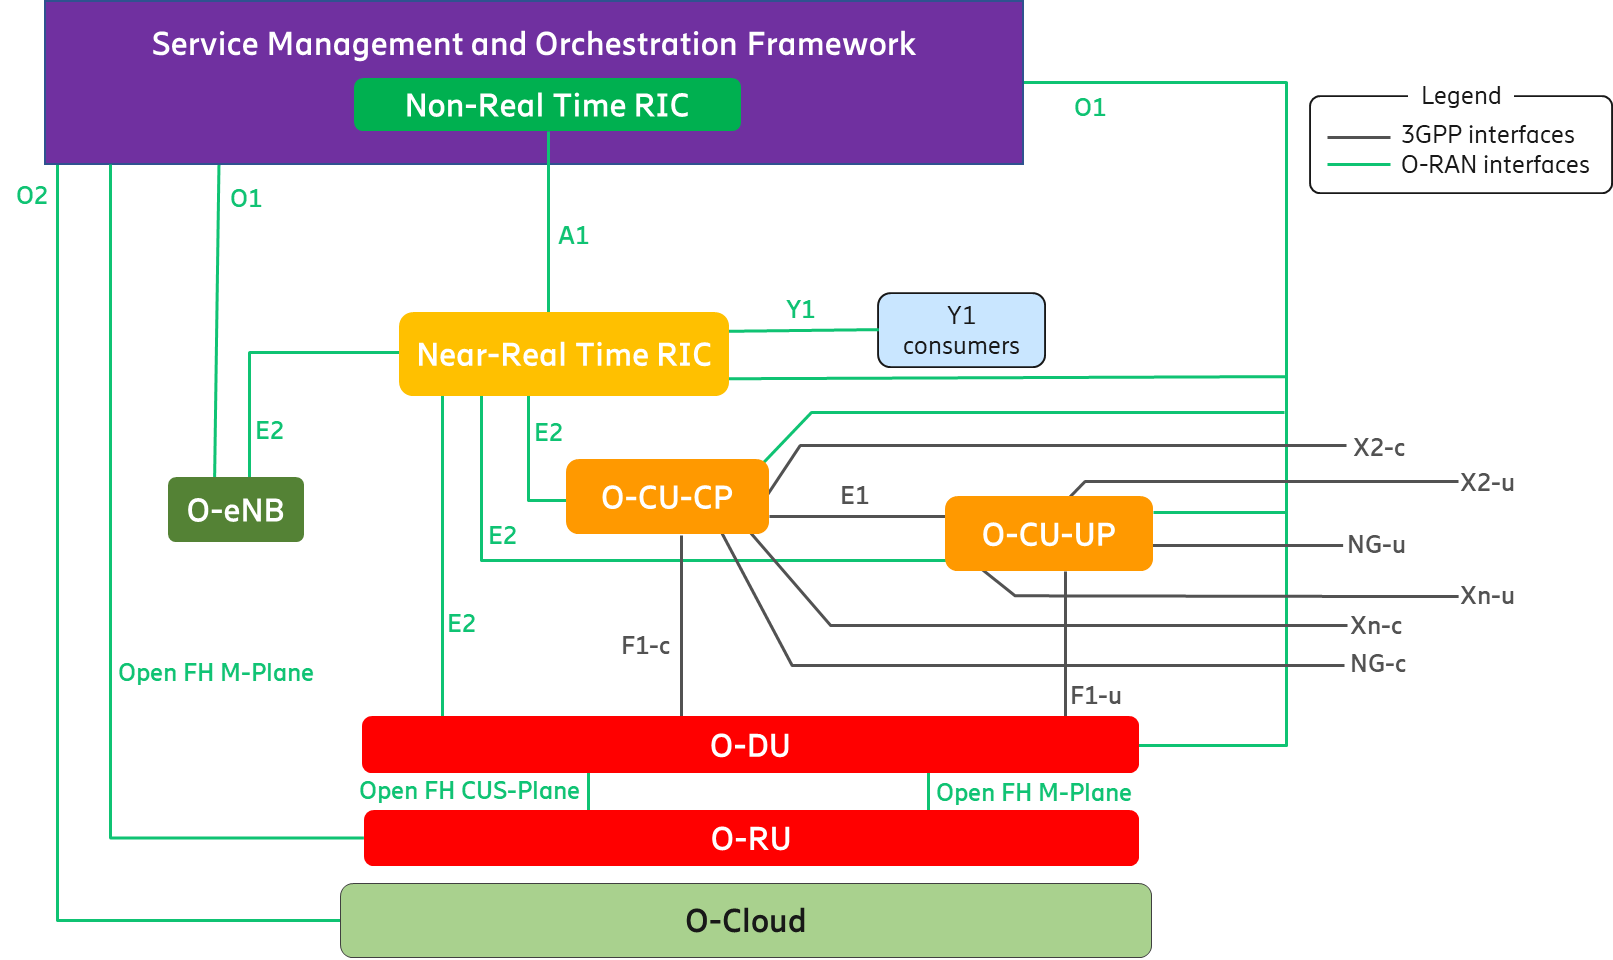
\includegraphics[width=0.8\textwidth]{oran-architecture}
    \caption{Logische Architektur von Open RAN (Quelle: \autocite{o-ranworkgroup1usecasesandoverallarchitectureORANArchitectureDescription})}
    \label{fig:oran-architecture}
\end{figure}
\section{5G-FORAN}
\label{sec:tech-foran}
\section{Dashboard}
\label{sec:tech-dashboard}


\chapter{Methodik}
\label{chap:methodik}
Die Methodik dieser Arbeit beschreibt das wissenschaftliche Vorgehen bei der Implementierung des Dashboards in einer \gls{dfir} Umgebung für O-RAN. Der Fokus liegt auf der Integration einer empirischen Methode zur Bewertung von Angriffen und der Weiterentwicklung passender Visualisierungstechniken.
\section{Theoretische Grundlagen der empirischen Methode}
\label{sec:auswahlDerEmpirischenMethode}
\gls{acema} ist \glqq{}eine umfassende empirische Methode zur Analyse von Bedrohungen in O-RAN Umgebungen\grqq{} (eigene Übersetzung: \autocite{klementSecuring6GTransition2024}). Die Integration der Analyse-Methode von \citeauthor{klementSecuring6GTransition2024} in das Forschungsprojekt \gls{foran} bringt wertvolle Daten ein, die nützliche Visualisierungen im Dashboard ermöglichen. Im Folgenden wird erläutert, welches Ziel mit der Integration von \gls{acema} verfolgt wird, welchen Mehrwert \gls{acema} für \gls{foran} bietet und wie die gewonnenen Daten angemessen im Dashboard visualisiert werden können.
\par \gls{acema} ermöglicht es, für spezifische \gls{mitre}-Techniken auf eine Menge an \glspl{cve} zu schließen. Das Ziel der Integration in diese Forschungsarbeit ist es, für spezifische simulierte Angriffe eine Bewertung nach dem \gls{cvss} vornehmen zu können. Die \gls{acema}-Arbeit hat, im Gegensatz dazu, nicht das Ziel spezifische Angriffe zu betrachten, sondern eine Übersicht über alle möglichen von der O-RAN definierten \textit{Threat-IDs} zu geben. Der generelle Vorgang ist in der Abbildung \ref{fig:mitre_mapping} dargestellt.

%
\begin{figure}
    \centering
    \begin{tikzpicture}[node distance=2cm, auto]
        % Nodes
        \node [rectangle, draw, text centered, minimum width=3cm] (mitre) {\textbf{\gls{mitre} - Technik}};
        \node [rectangle, draw, below of=mitre, yshift=-0.5cm] (capec) {\textbf{\gls{capec}}};
        \node [rectangle, draw, below of=capec, yshift=-0.5cm] (cwe) {\textbf{\gls{cwe}}};
        \node [rectangle, draw, below of=cwe, yshift=-0.5cm] (cve) {\textbf{\gls{cve}}};
        % Arrows
        \draw[->, thick] (mitre) -- (capec) node[midway, left] {Schritt 1: MITRE CTI};
        \draw[->, thick] (capec) -- (cwe) node[midway, right] {Schritt 2: MITRE CTI};
        \draw[->, thick] (cwe) -- (cve) node[midway, left] {Schritt 3: MITRE CWE Liste};
    \end{tikzpicture}
    \caption{Ablauf des Mappings von MITRE-Technik zu spezifischen CVE-Datum über die Kategorisierungssysteme MITRE, CAPEC, CWE und CVE.}
    \label{fig:mitre_mapping}
\end{figure}

\par Die spezifischen Angriffe, die im Dashboard angezeigt werden, stammen aus dem \gls{foran} \gls{at}. Das \gls{at} implementiert aktuell circa 250 Szenarien, die Angriffsspuren erzeugen. Diese werden im Dashboard in 45 Techniken\footnote{Wenn ohne Zusatz von einer Technik gesprochen wird, meint das im Rahmen dieser Arbeit eine Technik aus einer der drei in Kapitel \ref{sec:datenquellen} definierten Matrizen. Nur wenn ausdrücklich von einer \gls{mitre}-Technik oder \gls{mitre}-Taktik gesprochen wird, meint dies Inhalte des \gls{attack}-Frameworks.} sortiert und übergeordnet auf 10 Taktiken verteilt. Eine Technik kann dabei in mehreren Taktiken angewendet werden. Die Matrix im Dashboard orientiert sich stark an der \gls{tm4k}, da sich alle Angriffe des \gls{at}s einer Technik dieser Matrix zuordnen lassen. Für über 90\% der Techniken aus der \gls{tm4k} ist eine Zuordnung zu einer \gls{mitre}-Technik trivial möglich.
\par Schritt 1 des in Abbildung \ref{fig:mitre_mapping} dargestellten Ablaufs sucht für eine \gls{mitre}-Technik das zugehörige Angriffsmuster, den \gls{capec}. Die zugrundeliegenden Daten stammen aus dem von \gls{mitre} gepflegtem \gls{cti} Repository, in welchem die Daten regelmäßig aktualisiert veröffentlicht werden \autocite{MitreCtiCyber}. Die durch \gls{acema} gefundenen \glspl{capec} zu den \gls{mitre}-Techniken sind jedoch nicht vollständig, eine Erklärung und eine Lösung dafür wird in Kapitel \ref{sec:impl-anwendungVonAcema} präsentiert. Schritt 2 nutzt dasselbe Repository, dort sind für das jeweilige \gls{capec}-Objekt auch zugehörige \glspl{cwe} unter externen Referenzen verknüpft \autocite{CtiUSAGEmdMaster}. In Schritt 3 wird über das Pythonmodul \textit{cwe2} nach zugehörigen \glspl{cve} gesucht. Die zugrundeliegenden Daten für diese Abfrage stammen aus der \gls{cwe} Liste, die regelmäßig von \gls{mitre} veröffentlicht wird. Diese Liste enthält auch zugehörige \glspl{cve}, die in diesem Kontext \glqq{}beobachtete Beispiele\grqq{}\footnote{Auf Englisch: \glqq{}Observed Examples\grqq} genannt werden \autocite{AboutcodeorgCwe22024,CWEDownloads}. Um weitere Informationen wie \gls{cvss}, Angriffsvektoren und Veröffentlichungsdatum über einzelne \glspl{cve} zu beschaffen, wird die \gls{nvd} des \gls{nist}s über die Python Module \verb|cve_lookup| und \verb|nvdlib| abgefragt \autocite{NVDLibNVDLibNIST,MachineThingCve_lookupLook,NVDHome}.
\par Die Besonderheit an \gls{acema} in Vergleich zu anderen \gls{mitre}-Technik zu \gls{cve}-Mappingtools ist, dass eine tiefgründige Analyse in die betroffenen O-RAN Bedrohungen aus dem Report der \gls{wg11} möglich ist. Dazu ist im Vorhinein eine separate Zuordnung zwischen \gls{mitre}-Technik und O-RAN \textit{Threat-ID} aufzustellen.
\par Zusammenfassend müssen zwei Grundvoraussetzungen für die erfolgreiche Integration von \gls{acema} gegeben sein. Zum einen muss die Zuordnung einer oder mehrerer \gls{mitre}-Techniken zu einem Angriffsszenario des \gls{at}s gegeben sein. Zum anderen muss die Zuordnung einer \gls{mitre}-Technik zu einer oder mehreren O-RAN \textit{Threat-IDs} manuell erstellt werden.

\section{Grundprinzipien und Designentscheidungen für Visualisierungen}
\label{sec:auswahlDerVisualisierungstechniken}
Die Basis für die Wahl der Visualisierungstechniken im Dashboard wurden von Jonas Weber in seiner Arbeit gelegt \autocite{weberEvaluationDashboardTechniques}. \citeauthor{weberEvaluationDashboardTechniques} beschreibt darin grundlegende Prinzipien, die beim Design eines Dashboards eine wichtige Rolle spielen. Über das Design von Dashboards auf Basis dieses neurologischen Konzepts gibt es zahlreiche wissenschaftliche Arbeiten, hervorgehoben sei dabei die Literaturübersicht von \citeauthor{barrera-leonHowPreattentiveProcess2023} \autocite{barrera-leonHowPreattentiveProcess2023}. 
\par Das erste Prinzip beschreibt das Phänomen der präattentiven Wahrnehmung. Darunter versteht man die Wahrnehmung von visuellen Reizen, welche jedoch unterschwellig und ohne besondere Aufmerksamkeit geschieht. Man spricht auch von "Vorbewusstsein" \autocite{PraeattentiveWahrnehmung,mallotWahrnehmungPraeattentiveIm2021}. Anwendung findet dieses Prinzip in der Implementierung des Dashboards zum Beispiel beim Design der Zeitleiste. Im Listing \ref{fig:cvss-colors} ist dargestellt, wie der Schweregrad von Metriken eines \glspl{cve} anhand einer farblichen Kategorisierung eingeordnet wird. Die Farbwahl beschränkt sich hierbei auf vier deutlich voneinander unterscheidbaren Farben. Die Farbzuteilung ist in Tabelle \ref{tab:severity-color-mapping} dargestellt.
\begin{table}[H]
    \centering
    \caption{Farbzuordnung zu Schweregraden}
    \begin{tabular}{|c|c|}
        \hline
        \textbf{Farbe}                & \textbf{Schweregrad}  \\
        \hline
        \cellcolor[HTML]{6c757d} Grau & Keine Daten vorhanden \\
        \hline
        \cellcolor[HTML]{198754} Grün & Niedriger Schweregrad \\
        \hline
        \cellcolor[HTML]{ffc107} Gelb & Mittlerer Schweregrad \\
        \hline
        \cellcolor[HTML]{dc3545} Rot  & Hoher Schweregrad     \\
        \hline
    \end{tabular}
    \label{tab:severity-color-mapping}
\end{table}

Wissenschaftlich ist die kategorisierende Wahrnehmung von Farben unter anderem durch die wissenschaftliche Arbeit von \citeauthor{cliffordColorCategoriesAffect2010} bewiesen \autocite{cliffordColorCategoriesAffect2010}. Die technische Implementierung der Farbkategorisierung ist in Kapitel \ref{sec:impl-cvssIntegration} erläutert.
%
\begin{figure}
    \centering
    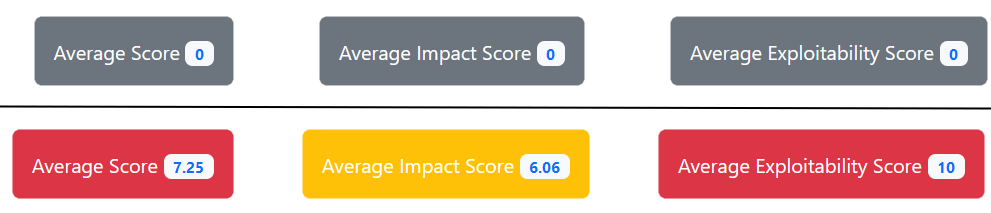
\includegraphics[width=0.8\textwidth]{cvss-colors}
    \caption{Farbkategorien zur Darstellung von Metriken}
    \label{fig:cvss-colors}
\end{figure}
%
\par Ein weiteres Prinzip, welches beim Visualisieren von Daten eine zentrale Bedeutung hat, wurde 1983 von \citeauthor{tufteBookReviewsVisual1984} als \textit{data-ink}-Prinzip definiert. Das Prinzip besagt, dass der Anteil der genutzten Farbe um die Daten darzustellen möglichst hoch sein soll. Damit soll die Darstellung von nicht-daten-bezogener Ausschmückung in der Visualisierung vermieden werden \autocite{tufteBookReviewsVisual1984}. An einem praktischen Beispiel kann jedoch gezeigt werden, dass ein geringeres \textit{data-ink} Verhältnis nötig sein kann, um Daten effizient darzustellen. Als zentrale zu visualisierende Daten eines Artefakts liegen jeweils das Start- und Enddatum vor. Die Abbildung \ref{fig:high-data-ink} zeigt die Darstellung von mehreren Artefakten auf einer Zeitleiste. Das \textit{data-ink} Verhältnis ist in dieser Darstellung sehr hoch, da tatsächlich nur die Start- und Endzeitpunkte dargestellt sind. Im Vergleich dazu wird in Abbildung \ref{fig:low-data-ink} die Zeitspanne zwischen den jeweiligen Daten eines Artefaktes zusätzlich farblich dargestellt. Es wird erkennbar, welche Punkte Start- oder Endpunkte sind. Dies war in Abbildung \ref{fig:high-data-ink} nicht intuitiv erkenntlich. Es ist in diesem Fall sinnvoll ein geringeres \textit{data-ink} Verhältnis zu erzielen, um Klarheit und Intuition zum Lesen zu schaffen. Die technische Konfiguration der Zeitleiste ist in Kapitel \ref{sec:impl-others} erläutert.
%
\begin{figure}
    \centering
    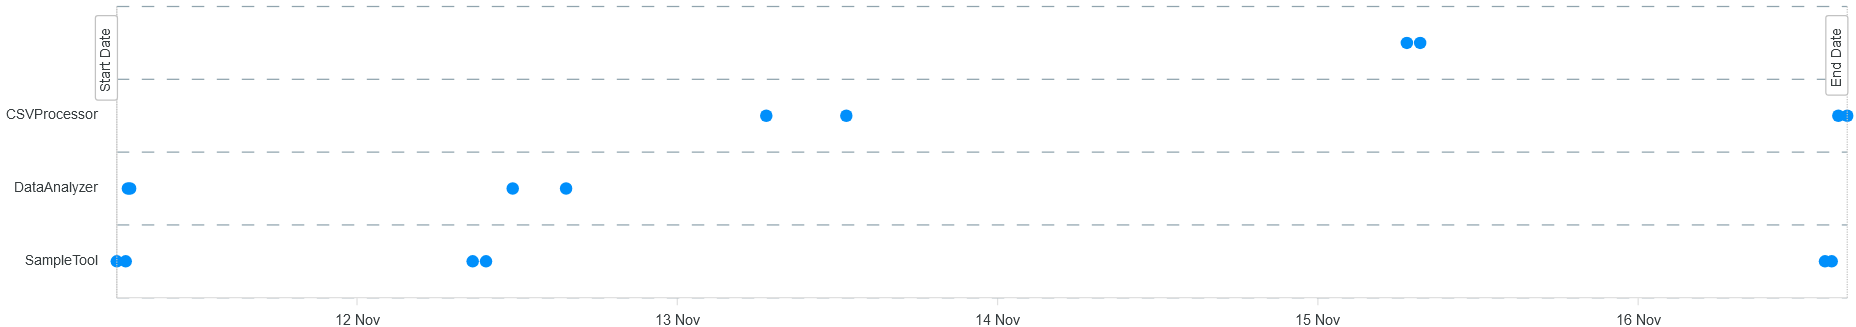
\includegraphics[width=1\textwidth]{high-data-ink}
    \caption{Hohes \textit{data-ink} Verhältnis}
    \label{fig:high-data-ink}
\end{figure}
%
\begin{figure}
    \centering
    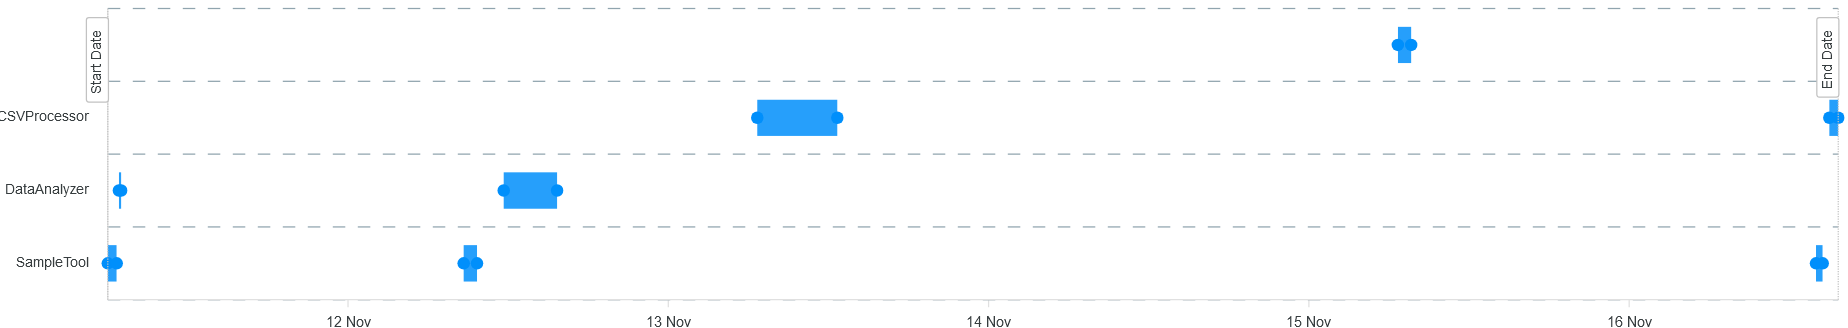
\includegraphics[width=1\textwidth]{low-data-ink}
    \caption{Niedriges \textit{data-ink} Verhältnis}
    \label{fig:low-data-ink}
\end{figure}
%
\par Diese beiden Prinzipien und andere Best Practices wurden auch bei Weiter- und Neuentwicklungen von Visualisierung im Dashboard gewahrt. Bei der Darstellung des Angriffspfads und der Netzwerktopologie wurden bewusste design-technische Entscheidungen getroffen. Die Angriffspfadsvisualisierung enthält nicht viele Daten, nimmt aber einen großen Platz auf der Detailübersicht eines Artefaktes ein. Ein gerichteter Graph bietet sich als Visualisierungstechnik an, da dieser leicht zu verstehen ist. Jedes Element im Graphen besitzt auch nur maximal eine Kante, die auf das nächste Element in der Kette des Angriffspfades steht. Der Angriffsgraph ist beim Laden der Seite nicht direkt, sondern nur nach einem bewussten Scrollen sichtbar. So wird der Nutzer\footnote{In dieser Arbeit wird aus Gründen der besseren Lesbarkeit das generische Maskulinum für eine Person verwendet, die das Dashboard nutzt. Alle Geschlechteridentitäten werden dabei ausdrücklich mitgemeint.} nicht mit zu vielen Informationen auf einmal überladen. Diese Entscheidung wird unterstützt durch die Studie von \citeauthor{toreiniDESIGNINGUSERADAPTIVEINFORMATION}, in der die Aufnahmefähigkeit in Verbindung mit der Anzahl von gleichzeitig sichtbaren Visualisierungen untersucht wird \autocite{toreiniDESIGNINGUSERADAPTIVEINFORMATION}.
\par Die Graphen werden nicht als statische Bilder eingebettet. So lassen sich weitere Funktionen wie Tooltips, dynamischer Zoom und die Neuanordnung der einzelnen Elemente durch den Nutzer realisieren. Ein Tooltip hat die Funktion, zusätzliche hilfreiche Information zu liefern, wenn der Nutzer mit dem Mauszeiger auf ein Element zeigt \autocite{TooltipCarbonDesign}. Die Darstellung eines Tooltips ist in Abbildung \ref{fig:tooltip} gezeigt. Über die Verschiebbarkeit der Elemente kann das Diagramm angepasst werden, um es verständlicher darzustellen oder für einen Export vorzubereiten. Die Graphen können über gängige Browser per \textit{Rechtsklick, Speichern unter / In neuem Tab öffnen} als \verb|.png| Datei exportiert werden. Die technische Implementierung des Angriffsgraphs, vom als Text definierten Graphen bis zur Visualisierung im Dashboard, und das Ergebnis der Implementierung sind in Kapitel \ref{sec:impl-visualisierungDesAngriffspfads} erläutert.
%
\begin{figure}
    \centering
    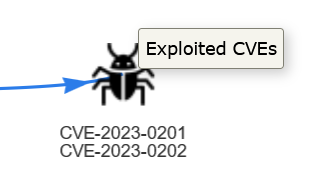
\includegraphics[width=0.5\textwidth]{tooltip}
    \caption{Tooltip auf einem Element im Angriffsgraph}
    \label{fig:tooltip}
\end{figure}
%
\section{Werkzeuge und Technologien}
\label{sec:Entwicklungsumgebung}
In diesem Kapitel wird etwas tiefer auf die Tools eingegangen, die zur Umsetzung der Implementierung des Dashboards genutzt wurden. Informationen über die generelle Architektur, genutzte Programmiersprachen und Technologien finden sich in Kapitel \ref{sec:tech-dashboard}.
\par Zu Beginn wurde die Entwicklung auf einer rein lokalen Umgebung durchgeführt. Über das von MongoDB zur Verfügung gestellte \gls{cli} lief ein MongoDB-Server, ein per \verb|go build| gebauter Dashboard-Server und der per \verb|yarn dev| gestartete Vite-Entwicklungs-Server auf dem lokalen Rechner \autocite{MongoDBDeveloperData,Vite}. Die Testdaten stammten aus dem Gitlab-Repository und wurden vom vorherigen Entwickler zur Verfügung gestellt \autocite{AddExampleData2023}. Die Qualität und Menge der Testdaten waren für den Anfang ausreichend. Der Testdatensatz wurde seitdem aktualisiert, um den aktuellen Stand der Daten zu repräsentieren, und kann über die MongoDB \gls{cli} mit \verb|mongoimport| geladen werden \autocite{JSONMongoDB}. Um mit aktuellen Daten zu arbeiten und näher an der etablierten Testumgebung zu sein, wurde ab dem 7. August 2024 eine \gls{vm} in der Umgebung des Labors für Datennetze (DN.Lab) der TH Köln genutzt. Die Anwendung konnte nun entweder weiterhin lokal auf der \gls{vm} oder zentralisiert per Ansible bereitgestellt werden \autocite{HomepageAnsibleCollaborative}. Ansible ist ein Tool zur Orchestrierung von Systemen und Software, welches durch die Ausführung von Skripten einen spezifischen technischen Zustand herstellt \autocite{ansiblecollaboratorsHowAnsibleWorks2024}. Für die Ausführung des \gls{acema}-Quellcodes ist das Aufsetzen einer Python-Umgebung nötig \autocite{klement2023acema,WelcomePythonorg}. Bei der Implementierung des Dashboards wurde für die Entwicklung und das Debugging gelegentlich ChatGPT-4o von OpenAI genutzt, um allgemeine Programmierfragen zu klären und Unterstützung bei Bearbeitung von repetitiven Aufgaben zu erhalten.
\chapter{Implementierung}
\label{chap:implementierung}
In diesem Kapitel wird die praktische Umsetzung der im Methodikteil beschriebenen Ansätze detailliert erläutert. Der Schwerpunkt liegt dabei auf der Anwendung und Integration der empirischen Methode \gls{acema}. Außerdem wird beschrieben, wie und wo die Integration von \gls{cvss} Daten vorgenommen wurde. Weiterhin wird auf die Visualisierung des Angriffspfads eingegangen und erklärt, welche Tools dafür eingesetzt wurden. Abschließend werden zusätzliche Implementierungen vorgestellt, die die Funktionalität und Benutzerfreundlichkeit des Dashboards erweitern, darunter die Verbesserung der Zeitleistenansicht, die Vereinfachung der Datenstruktur von Artefakten sowie weiterführende Informationen zu genutzten Techniken.
\par Grundlegend besitzt das Dashboard vier verschiedene Seiten, die aus dem Hauptmenü angesteuert werden können. Die Seiten von Artefakten und Kampagnen sind dabei in die Übersichtsseite und die Detailsansicht zu trennen, \gls{acema} und Matrix besitzen nur die Hauptroute. In der folgenden Übersicht sind alle Routen dargestellt, die im Dashboard verfügbar sind. Angegeben wird auch, welche Daten verwendet werden, um die Seite dynamisch mit Inhalt zu füllen.

\begin{itemize}
    \item \textbf{/ (Startseite):} Statische Startseite des Dashboards mit Buttons zur Navigation zu anderen Routen.
    \item \textbf{/acema (Darstellung der ACEMA Diaramme):} Enthält alle über ACEMA erstellen Diagramme als PDFs.
    \item \textbf{/mitre/kubernetes\_matrix (Kubernetes Matrix):} Visualisierung der angepassten \gls{mitre} \gls{attack} Matrix.
          \begin{itemize}
              \item \textbf{Dynamisch erzeugt aus:}
                    \begin{itemize}
                        \item \textbf{kubernetes\_matrix.tmpl:} Nutzt die Anzahl der Taktiken und Techniken zum Aufbau der Zeilen und Spalten.
                        \item \textbf{technique.partial.tmpl:} Füllt die Felder mit den in  \\
                        \verb|pkg/mitre/technique.go| definierten Techniken.
                    \end{itemize}
          \end{itemize}

    \item \textbf{/artifacts (Artefakte - Index):} Liefert eine Liste aller Artefakte, aller Filtermöglichkeiten und einer visuellen Darstellung auf der Zeitachse.
          \begin{itemize}
              \item \textbf{Query-Parameter (optional):}
                    \begin{itemize}
                        \item \texttt{tool\_name} - Filtert Artefakte nach dem Namen des Tools.
                        \item \texttt{tactic} - Filtert Artefakte nach der zugehörigen Taktik.
                        \item \texttt{microsoft\_technique} - Filtert Artefakte nach Microsoft-Techniken.
                        \item \texttt{start\_date} - Filtert Artefakte nach Startzeitpunk.
                        \item \texttt{end\_date} - Filtert Artefakte nach Endzeitpunkt.
                    \end{itemize}
              \item \textbf{Dynamisch erzeugt aus:}
                    \begin{itemize}
                        \item \textbf{artifacts/index.tmpl:} Nutzt die Daten aller Artefakte und die Werte der Filterparameter.
                    \end{itemize}
          \end{itemize}

    \item \textbf{/artifacts/:id (Artefakte - Details):} Liefert Details zu einem spezifischen Artefakt anhand der \texttt{id}.
          \begin{itemize}
              \item \textbf{Dynamisch erzeugt aus:}
                    \begin{itemize}
                        \item \textbf{artifacts/show.tmpl:} Nutzt die Daten eines Artefaktes.
                        \item \textbf{error.tmpl:} Spezifische Fehlermeldung von Go nach Datenbankabfrage.
                    \end{itemize}

          \end{itemize}

    \item \textbf{/campaigns (Kampagnen - Index):} Liefert eine Liste aller Kampagnen.
          \begin{itemize}
              \item \textbf{Dynamisch erzeugt aus:}
                    \begin{itemize}
                        \item \textbf{campaigns/index.tmpl:} Nutzt die Daten aller Artefakte und die Werte der Filterparameter.
                    \end{itemize}
          \end{itemize}

    \item \textbf{/campaigns/:id (Kampagnen - Details):} Liefert Details zu einer spezifischen Kampagne anhand der \texttt{id}.
    \begin{itemize}
    \item \textbf{Query-Parameter (optional):}
          \begin{itemize}
              \item \texttt{start\_date} - Filtert Kampagnen nach Startzeitpunk.
              \item \texttt{end\_date} - Filtert Kampagnen nach Endzeitpunkt.
          \end{itemize}
    \item \textbf{Dynamisch erzeugt aus:}
            \begin{itemize}
                \item \textbf{campaigns/show.tmpl:} Nutzt die Daten einer Kampagne.
                \item \textbf{error.tmpl:} Spezifische Fehlermeldung von Go nach Datenbankabfrage.
            \end{itemize}
    \end{itemize}
\end{itemize}

\section{Implementierung von ACEMA}
Die empirische Methode kann auf zwei verschiedenen Arten für das Dashboard genutzt werden. Zum einen lassen sich über die Matrixdaten aus Anhang \ref{app:mapping-dataset} sehr aussagekräftige Diagramme erstellen, die jedoch nicht direkt in die Technik- oder Artefaktdarstellung im Dashboard integriert werden. Zum anderen gibt der Output von \gls{acema} die Möglichkeit, die \gls{cvss} Daten direkt in existierende Seiten des Dashboards zu integieren und den Inhalt aufzuwerten.

\subsection{Anwendung von ACEMA auf die Daten}
\label{sec:impl-anwendungVonAcema}
Der allgemeine Ablauf der Mappings wurde in Kapitel \ref{sec:auswahlDerEmpirischenMethode} bereits angeschnitten. Es wurden zwei Grundvoraussetzungen definiert, die für die erfolgreiche Implementierung von \gls{acema} nötig sind. Die erste Voraussetzung (Zuordnung Angriffsszenario zu \gls{mitre}-Technik) wurde von den Verantwortlichen des \glspl{at} umgesetzt. Die zweite Voraussetzung bedurfte einer manuellen Zuordnung von Techniken zu O-RAN \textit{Threat-IDs}. Diese Zuordnung ist einmal manuell nötig und aufgrund der ausführlichen Beschreibungen der Techniken und \textit{Threat-IDs} gut machbar. Diese Zuordnung ist in die Datenstruktur einer Technik im Dashboard integriert. Eine Technik in der modifizierten Matrix wird wie in Listing \ref{list:def-technique} beispielhaft gezeigt definiert.
\begin{code}[caption=Beispielhafte Definition einer Technik im Dashboard, label={list:def-technique}]
    AddEntryToMap(
        "MS-TA9002",                        // KEY in die Map
        "MS-TA9002",                        // TM4K-ID
        []string{"T1195.002", "T1525"},     // ATT&CK-Technik-IDs
        "Compromised Image In Registry",    // Technik Name
        []string{"initial-access"},         // ATT&CK-Taktik-Namen
        []string{"T-IMG-01"},               // O-RAN Threat-IDs
    )
\end{code}

Ein Export im \verb|csv| Format aller definierten Techniken ist in Anhang \ref{app:mapping-dataset} abgebildet. Dieser Datensatz stellt auch gleichzeitig die Eingangsdatei dar, auf dessen Basis \gls{acema} arbeitet. Der Datenexport wird erzeugt, wenn die Dashboardanwendung gestartet wird.
\par Die Implementierung von \gls{acema} lässt sich in zwei Teile spalten: den \verb|Gathering|-Teil (deutsch: Sammlungsteil) und den \verb|Analysis|-Teil (deutsch: Analyseteil). Es existieren hierfür jeweils eine Datei mit den aufrufbaren Funktionen und eine andere, die die Aufrufe dieser Funktionen tätigt und prozedural ausgeführt wird.

\par Es wurden einige Anpassungen des verfügbaren \gls{acema}-Quellcodes vorgenommen, die den Entwicklungsfluss vereinfachen und Verbesserungen vornehmen. Eine vorgenommene Verbesserung bezieht sich auf die Vollständigkeit des Daten-Mappings. Es wird in Kapitel \ref{sec:limitationen} gezeigt, dass die im Folgenden beschriebene Verbesserung zu der Schöpfung einer größeren Datenmenge aus dem \gls{cti} Repository führt. Eine weitere Änderung betrifft die Ausführung der Python Skripte. Die prozeduralen Teile sind im originalen Repository als \verb|jupyter notebooks| (\verb|.ipynb|-Dateien) geschrieben \autocite{klement2023acema,ProjectJupyter}. Diese Dateien wurden zu einfacheren Ausführung in \verb|.py| Dateien konvertiert, sodass sie direkt über die Python-\gls{cli} aufrufbar sind. Eine Ausführung in einem Jupyter Notebook ergibt für das erstmalige Nachvollziehen oder Demonstrationszwecke Sinn, ist aber für die spätere Ausführbarkeit hinderlich.
\par Informationen über alle genutzten Quellcodes in dieser Arbeit und wo diese zu finden sind, werden ein Anhang \ref{app:sourcecode} zur Verfügung gestellt.

Der originale Quellcode arbeitet beim Mapping von \gls{mitre}-Technik zu \gls{capec} mit einem \textit{pandas dataframe}. Pandas ist eine bekannte Datenanalysebibliothek für Python \autocite{PandasPythonData}. Für das Konvertieren von \gls{stix}-Daten zu einem \textit{dataframe} wird die Funktion \verb|mitreattack.stixToDf| genutzt \autocite{MitreattackpythonMitreattackAttackToExcel}. Es wird dadurch der \textit{enterprise-attack}-Teil der \gls{cti} Daten durchsucht. Viele Beziehungen zwischen \gls{mitre}-Technik und \gls{capec} finden sich jedoch auch im \textit{capec/2.1/attack-pattern} Teil des Repositories. Diese Limitation bringt signifikant weniger Mappings zum Vorschein, wie empirisch in Kapitel \ref{limitationen-acema} gezeigt wird. Deshalb nutzt die verbesserte Implementierung die Datensätze aus beiden Teilen. Auch wurde ein anderer Ansatz zur Verarbeitung der einzelnen \verb|json|-Dateien angewandt. Anstatt der Konvertierung zu einem mächtigen \textit{dataframe} der alle Daten enthält, werden die \gls{stix}-Daten aus jeder \verb|json|-Datei einzeln geladen und der Inhalt der \gls{stix}-Objekte über \verb|stix_data.get()| ausgelesen \autocite{OasisopenCtipythonstix2OASIS}. Die genaue Abfolge der abgefragten Kriterien bis zum Finden eines Mappings in Abbildung \ref{fig:detailed-mapping} ist als detaillierte Ansicht des Schrittes 1 in Abbildung \ref{fig:mitre_mapping} zu verstehen.

\usetikzlibrary{shapes.geometric, arrows}
\tikzstyle{startstop} = [rectangle, rounded corners, minimum width=0cm, minimum height=0cm, text centered, draw=black, fill=red!30]
\tikzstyle{process} = [rectangle, minimum width=0cm, minimum height=0cm, text centered, draw=black, fill=blue!30]
\tikzstyle{decision} = [diamond, minimum width=0cm, minimum height=0cm, text centered, draw=black, fill=green!30]
\tikzstyle{arrow} = [thick,->,>=stealth]

\begin{figure}
    \centering
    \begin{tikzpicture}[node distance=2.5cm and 3cm]

        % Nodes for processes and start
        \node (start) [startstop] {Start (Loop through Directories)};
        \node (loadJson) [process, below of=start] {Load and Parse JSON};
        \node (processObjects) [process, below of=loadJson] {Process Objects in JSON};
        \node (extractCapec) [process, below of=processObjects, yshift=-7cm] {Extract CAPEC Reference};
        \node (appendCapec) [process, below of=extractCapec] {Append CAPEC ID to Results};

        % Nodes for decisions (aligned left)
        \node (checkType) [decision, left of=start, xshift=-5cm, yshift=-3cm] {Is Object Type `attack-pattern`?};
        \node (checkRef) [decision, below of=checkType, yshift=-5cm] {Is `source\_name` = `capec`};
        \node (checkTechnique) [decision, below of=checkRef, yshift=-5cm] {`external\_id` in Techniques?};

        % Node for Stop and finish
        \node (end) [startstop, right of=checkRef, xshift= +5cm] {End Loop};
        \node (finish) [startstop, below of=appendCapec] {Finished};


        % Arrows from processes to decisions
        \draw [arrow] (processObjects.west) -- (checkType.east);
        \draw [arrow] (start) -- (loadJson);
        \draw [arrow] (loadJson) -- (processObjects);

        % Arrows between decisions
        \draw [arrow] (checkType) -- node[anchor=east] {Yes} (checkRef);
        \draw [arrow] (checkRef) -- node[anchor=east] {Yes} (checkTechnique);

        % Arrows for "No" to End Loop
        \draw [arrow] (checkType.south east) -- node[anchor=east] {No} (end.west);
        \draw [arrow] (checkRef.east) -- node[anchor=east] {No} (end.west);
        \draw [arrow] (checkTechnique.north east) -- node[anchor=east] {No} (end.west);

        % Arrow from last decision to process
        \draw [arrow] (checkTechnique.east) -- node[anchor=east] {Yes} (extractCapec.west);

        % Arrow from processes to the next
        \draw [arrow] (extractCapec) -- (appendCapec);
        \draw [arrow] (appendCapec) -- (finish);

    \end{tikzpicture}
    \caption{Detailansicht des Ablaufs des Mappings von MITRE-Technik zu CAPEC.}
    \label{fig:detailed-mapping}
\end{figure}

Wenn alle Mappings über die verbesserte Implementierung gefunden wurden, werden die Ergebnisse mit den Ergebnissen aus der originalen Implementierung zusammengeführt. Dadurch ergibt sich das komplette Mapping von \gls{mitre}-Technik zu \gls{capec}. Für die anderen Schritte des Mappings wurden keine Verbesserungsmöglichkeiten gefunden, daher sind die Funktionen aus dem originalen Quellcode beibehalten worden. Die Ausgabe der \gls{acema} Ausführung ist eine Datei im \verb|json| Format. Ein beispielhafter Auszug aus dieser Datei ist im Anhang \ref{app:acema-output} dargestellt. Bis zur Erstellung dieser Datei vergingen beim letzten Durchlauf knapp unter 40 Minuten. Das ist der hohen Anzahl der \glspl{cve} geschuldet, für die jeweils eine Anfrage an die \gls{nvd} geschickt wird. Die Dokumentation der \gls{nvd} Schnittstelle empfiehlt eine Wartezeit von sechs Sekunden zwischen Anfragen \autocite{DevelopersStartHere}.
\[353 \text{ CVEs} \cdot 6 \text{ Sekunden Wartezeit} \thickapprox 35 min \]

Der Output des \textit{Gathering} Skripts wird für die Analyse der Daten verwendet, um verschiedene Arten von Diagrammen zu erzeugen. Auf die Erkenntnisse, die man aus diesen Diagrammen gewinnen kann, wird in Kapitel \ref{sec:interpretation-acema} eingegangen. Alle Diagramme können auch im Dashboard angezeigt werden. Dazu wurde die Seite \verb|/acema| erstellt, die alle pdf-Dateien aus dem Ordner \verb|public\data| enthält. Neben den von \citeauthor{klementSecuring6GTransition2024} erstellten Diagrammen wurden einige weitere implementiert, die tiefere Einsicht in die Daten geben. Die Erstellung zusätzlicher Diagramme wird durch die Nutzung bekannter Datenanalyseframeworks und die umfangreiche Dokumentation im Quellcode unterstützt.

\par Aktuell ist es nicht implementiert, die \gls{acema} Python Skripte aus dem Dashboard heraus auszuführen, um eine neue Datensammlung oder Datenauswertung zu starten. Die Änderungsrate der Daten ist zudem eher gering, insofern ist eine Aktualisierung in kleinen Abständen nicht nötig. Die \gls{mitre}-Techniken im Dashboard sind quasi statisch, da sie sich an den implementieren Szenarien des \glspl{at} und dem \gls{attack}-Framework in Version \textit{16.1} orientieren. Insgesamt umfasst die Gesamtmenge aller \glspl{capec} 559 in \gls{capec} Version \textit{3.9}, wobei seit Januar 2023 nur vier neue (\(+0{,}7\%\)) hinzugefügt wurden. Auch die Veränderung im Mapping zwischen \gls{capec} und \gls{cwe} ist gut dokumentiert auf der \gls{capec} Webseite einsehbar. Hier ist eine Veränderung von 59 neu hinzugefügten Mappings in Version \textit{3.9} vor dem Hintergrund der Gesamtmenge auch eine sehr kleine Veränderung. Die Gesamtmenge der \gls{capec}-zu-\gls{cwe}-Mappings lässt sich anhand folgender Daten aus dem Testdatensatz in Anhang \ref{app:mapping-dataset} und dem Wert aus \autocite{CAPECNewsEvents} schätzen:
\[
    \begin{alignedat}{2}
         & \text{Anzahl von CAPEC in Testdatensatz}            & \quad & = 29             \\
         & \text{Anzahl von CWE in Testdatensatz}              & \quad & = 119            \\
         & \text{Durchschnittliche Anzahl von } \frac{\text{CWEs}}{\text{CAPEC}} & \quad & =
        4{,}1                                                                                              \\
        & \text{Gesamtmenge aller CAPECs}                        & \quad & = 559 \\
        & \text{Schätzung der Anzahl der Mappings}                             & \quad & =
         559 \cdot 4{,}1                                                  \\
         &                                                                      &       & \thickapprox2300 \\
    \end{alignedat}
\]
Zu einem ähnlichen Wert von 1700 bis 2800 kommt auch OpenAI ChatGPT 4o, wobei dort mit Werten von 3 bis 5 für die Anzahl der durchschnittlichen \glspl{cwe} pro \gls{capec} gerechnet wird \autocite{openaichatgpt4oCAPECCWEMapping2024}.

Zuletzt muss noch das Mapping von \gls{cwe} zu \gls{cve} betrachtet werden. Die Daten dazu stammen aus der \gls{mitre} \gls{cwe} Liste und werden mehrmals jährlich, ungefähr alle vier Monate aktualisiert \autocite{CWEDownloads,AIWorkingGroupMeeting_slides20241115_CWEAIWGpdf2024}.

Das Mapping zwischen \gls{mitre}-Technik und \glspl{cve} ändert sich infolgedessen nur in geringer Weise. Eine Integration der neuen Daten durch das Ausführen der \gls{acema} Skript und das Kopieren der \verb|json|-Datei in die Dashboardverzeichnisse \verb|pkg\artifacts| und \verb|pkg\mitre| ist demnach nicht kontinuierlich, aber mit einem Abstand von ungefähr vier Monaten, angepasst an die Änderungsrate der \gls{cwe} Liste, empfehlenswert.

\label{sec:impl-cvssIntegration}
Eine Integration mit dem \gls{cvss} ist eine grundlegende Funktion für jede Anwendung, die eine Bewertung von Schwachstellen vornimmt. Der \gls{cvss} Wert hilft dabei, schnell einen Überblick über den Schweregrad eines potenziellen Angriffs durch Ausnutzung der spezifischen Schwachstelle zubekommen. Aus diesem Grund hatte die Umsetzung von Beginn an eine hohe Priorität. Ursprünglich sollte die Bewertung nur über manuell zugeordnete \glspl{cve} vorgenommen werden, dieser Ansatz stellte sich allerdings als mühsam und nicht praktikabel heraus. Über die in Kapitel \ref{sec:impl-anwendungVonAcema} beschriebene Implementierung von \gls{acema} war eine deutlich schnellere und automatisierte Anreicherung von Daten mit \glspl{cve} möglich. Die Visualisierung von spezifischen Werten, die sich aus insgesamt sechs \gls{cvss} Metriken zusammensetzen, wurde an zwei Stellen implementiert, die im Folgenden genauer betrachtet werden.
Der in Listing \ref{list:go-embed} dargestellte und im nachfolgenden Kapitel beschriebene Go Quellcode arbeiten nicht direkt mit dem originalen Output von \gls{acema} (Dateiname: \verb|t-cwe-cve-dict.json|), sondern mit einer eigens leicht abgewandelten Version, in der nur die für das Dashboard relevanten Daten vorhanden sind. Der abgewandelten Quellcodes sind im Fork \autocite{jesseDumpeldownAcema_oranDev} des Repositories \autocite{klement2023acema} verfügbar. Diese \textit{neue} Datei mit dem Suffix \textit{\_small} wird über das Ausführen von \verb|data_analysis_nb.py| erstellt. Darin sind nur die Daten enthalten, die für die Integration einer Bewertung nach \gls{cvss} nötig sind, wie in Anhang \ref{app:acema-output-small} zu erkennen ist. Die enthaltenen Daten beschränken sich auf \gls{mitre} Technik-ID, \gls{capec}-ID, \gls{cwe}-ID, \gls{cve}-ID, und vier Metriken aus zwei Metrikgruppen die in \gls{cvss}Version 2 definiert sind \autocite{CVSSV2Complete}. Weiterführende Information über Metrikgruppen finden sich im Folgenen.

\par Um die Outputdatei mit den relevanten Daten im Dashboard nutzen zu können, wird das Paket \verb|embed| aus der Standard Bibliothek von Go genutzt \autocite{EmbedPackageEmbed}. Dies ermöglicht es, auf die Datei zuzugreifen, nachdem das Dashboard Projekt mit \verb|go build cmd/main.go| zu einer Binärdatei kompiliert wurde. Der Quellcode in Listing \ref{list:go-embed} zeigt, wie die Datei in eine Variable gelesen wird, die ein lokales Dateisystem simuliert. Von dort kann die Datei in Objekt in die vorher definierte Liste vom Datentyp \verb|ACEMA_DATA| gelesen werden. Die Variable \verb|ACEMA_DATA.Data| agiert hierbei quasi als \textit{Immutable Object} (deutsch: unveränderliches Objekt), das heißt der Wert der Datei wird während der Laufzeit einmal gesetzt und nicht mehr verändert. Die Sprache Go hat keinen eingebauten unveränderlichen Datentyp, der die bei Laufzeit gesetzt werden kann. Außerdem wird die Datei nicht unnötig aus dem Speicher gelesen, wenn die Daten bereits in der Variable vorhanden sind. Die Datenstruktur folgt daher dem \gls{worm}-Prinzip. Ausgelesen werden die Daten mehrfach während der Visualisierung der \gls{cvss} Daten.

\begin{code}[caption=Datei in Binardatei einbetten und in Struktur überführen, label={list:go-embed}]
    //go:embed t-cwe-cve-dict-small.json
    var data_json embed.FS
    if ACEMA_DATA.Data == nil {
        fileData, err := data_json.ReadFile("t-cwe-cve-dict-small.json")
        if err != nil {
                log.Fatal(err)
            }
        err = json.Unmarshal(fileData, &ACEMA_DATA.Data)
        if err != nil {
                log.Fatal(err)
            }
    }
\end{code}


Die Visualisierung von einem durchschnittlichen\footnote{In diesem Kapitel wird über den Durchschnitt von Werten gesprochen, gemeint ist immer das arithmetische Mittel.} \gls{cvss} Wert für eine \gls{tm4k}-Technik in der Matrix ist einer der Anwendungszwecke, die durch das von \gls{acema} erstellte Mapping möglich gemacht wird. Dabei wird für eine Technik der Durchschnitt aller \gls{cvss} \textit{v2\_score} Werte in den zugeordneten \glspl{cve} gebildet (siehe Zeile 1 im Listing \ref{list:mean}).  Wie bereits in Kapitel \ref{limitationen-acema} beschrieben, nutzt \gls{acema} das \gls{cvss} in Version 2. Die Metrik \textit{v2\_score} ist dabei ein Wert, der sich aus allen vorhandenen Metriken aus den verschiedenen Metrikgruppen zusammensetzt. In der \textit{Gruppe der Basismetriken} werden die grundlegenden Merkmale einer Schwachstelle bewertet, die sich, im Gegensatz zu Metriken aus der \textit{zeitlichen Gruppe} und der \textit{Umgebungsgruppe}, nicht über die Zeit verändern \autocite{CVSSV2Complete}.

Bei der Ausführung von \verb|data_analysis_nb.py| wird auch für jede \gls{mitre}-Technik die Berechnung der durchschnittlichen \gls{cvss} Werte über alle gefundenen \glspl{cve} durchgeführt. In der Funktion \verb|generate_json_with_scores| werden dazu die jeweiligen Werte in einer Liste gesammelt und mithilfe der Funktion \verb|mean(list[])| aus dem Python Modul \verb|statistics| das arithmetische Mittel berechnet, wie in Listing \ref{list:mean} gezeigt.
\begin{code}[caption=Berechnung des arithmetischen Mittels aus den CVSS Metriken mehrerer CVEs, label={list:mean}]
    new_technique["avg_score"] = statistics.mean(all_v2_scores)
    new_technique["avg_impact_score"] = statistics.mean(all_v2_impact_scores)
    new_technique["avg_exploitability_score"] = statistics.mean(all_v2_exploitability_score)
\end{code}

Die arithmetischen Mittel der Metriken werden daher somit direkt in die \verb|json|-Datei geschrieben und müssen nicht bei einem Neustart des Dashboards neu berechnet werden.

Eine visuelle Darstellung der Berechnung des \textit{Basisscores} ist in Abbildung \ref{fig:calc-cvss} gezeigt. Zu ungefähr 90\% der im Dashboard dargestellten Techniken ist eine \gls{mitre}-Technik zugeordnet und über \gls{acema} können für diese insgesamt 306 relevante \glspl{cve} gefunden werden. Diese Menge an \glspl{cve} bietet eine ausreichende wissenschaftliche Basis zur Auswertung von \gls{cvss} Daten. Es sind keine zu visualisierende Daten verfügbar, wenn entweder keine \glspl{cve} zu der \gls{mitre}-Technik gefunden werden oder keine \gls{mitre}-Technik zu der Technik im Dashboard zugewiesen ist. Drei Beispiele sind in Abbildung \ref{fig:technik-vis-example} abgebildet. Die gesamte Matrix mit allen Zuordnungen und \gls{cvss} Werten ist im Anhang \ref{app:matrix} dargestellt.

\begin{figure}
    \centering
    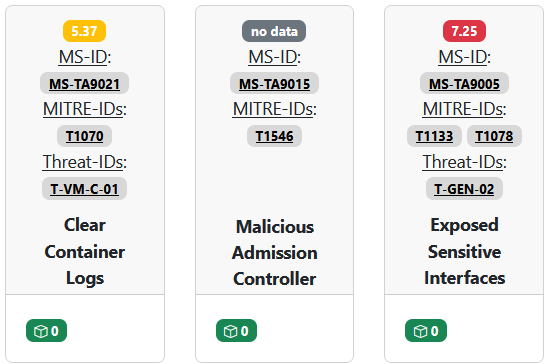
\includegraphics[width=0.6\textwidth]{technik-vis-example}
    \caption{Visualisierung des Basiswerts für eine Technik}
    \label{fig:technik-vis-example}
\end{figure}


\begin{figure}
    \centering
    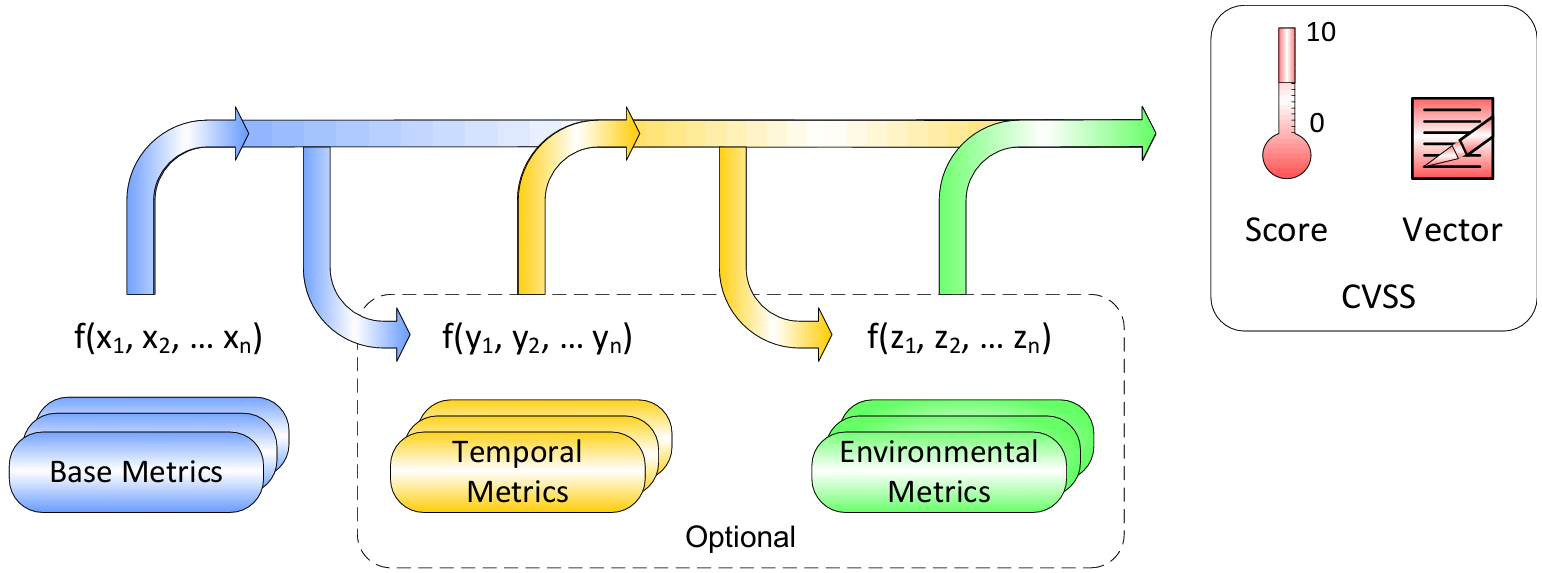
\includegraphics[width=0.8\textwidth]{calc-cvss}
    \caption{Einflüsse in der Berechnung des CVSS \textit{Basisscores} über die drei Metrikgruppen}
    \label{fig:calc-cvss}
\end{figure}

\par Eine weitere Anwendung findet die Integration mit \gls{cvss} Daten in der Übersichtsseite eines Artefakts. Die dort angezeigten Werte sind auch wieder Durchschnittswerte, die sich aus den \glspl{cve} zusammensetzen, die genau der einen \gls{mitre}-Technik in diesem Artefakt zugeordnet wurden. Zusätzlich zu dem generellen Durchschnittswert wird in der Detailansicht zwei weitere Wert dargestellt, der die Auswirkung und die Ausnutzbarkeit der zugeordneten \glspl{cve} darstellt. Einer der Werte setzt sich auf drei der Metriken aus der  \textit{Gruppe der Basismetriken} zusammen. Alle \textit{Impact} (deutsch: Auswirkung) Metriken werden zu einem \textit{v2\_impact\_score} zusammengefasst. Der andere Wert stammt aus der zeitlich veränderlichen Metrikgruppe und beschreibt die \textit{Exploitability} (deutsch: Ausnutzbarkeit) der Schwachstelle \autocite{CVSSV2Complete}. Die Bewertung der Ausnutzbarkeit verändert sich zum Beispiel, wenn ein Update für die angreifbare Software veröffentlich wird, die die Sicherheitslücke schließt.
Über die Darstellung der Werte wird eine gute Übersicht der Schwere einer Schwachstelle gegeben. Nach dem Basisscores sind die Angabe der Bewertung der Ausnutzbarkeit und der Auswirkungen die gängigsten Matriken. Die Berechung dieser Werte wird durch die folgenden Formeln ausgedrückt:

\begin{align*}
    \text{Auswirkungen}    & = 10{,}41 \cdot \Big( 1
    - (1 - \text{Vertraulichkeitsverlust}) \notag                                      \\
                           & \quad \cdot (1 - \text{Integritätsverlust})
    \cdot (1 - \text{Verfügbarkeitsverlust}) \Big) \notag                              \\[10pt]
    \text{Ausnutzbarkeit}  & = 20 \cdot \text{Angriffsvektor}
    \cdot \text{Angriffskomplexität} \notag                                            \\
                           & \quad \cdot \text{Authentifizierung} \notag               \\[10pt]
    f(\text{Auswirkungen}) & =
    \begin{cases}
        0,       & \text{wenn Auswirkungen} = 0, \\
        1{,}176, & \text{sonst.}
    \end{cases}                                           \\
    \text{Basisscore}      & = \text{Runden auf 1 Dezimalstelle} \Bigg[ \Big(
    (0{,}6 \cdot \text{Auswirkungen}) \notag                                           \\
                           & \quad + (0{,}4 \cdot \text{Ausnutzbarkeit}) - 1{,}5 \Big)
    \cdot f(\text{Auswirkungen}) \Bigg] \notag                                         \\[10pt]
\end{align*}

\par In beiden Fälle ergänzt eine farbliche Darstellung die numerischen Werte. Die Implementierung im Go Quellcode ist in Listing \ref{list:scorecolor} gezeigt. Die Schwellwerte, die ein Spektrum zu einer diskreten Farbe abbilden, können hier angepasst werden. Diese Funktion wird dann über die \verb|template.FuncMap| als Funktion definiert, die direkt in einer \verb|.tmpl| Datei genutzt werden kann. \textit{Go Templates} (deutsch: Vorlagen) werden in Go genutzt, um datengesteuert \gls{html}-Seiten mit dynamischen Daten aus einer Datenquelle zu befüllen. Die Datenquellen sind in der Implementierung des Dashboards Objekte oder eine Liste von Objekten vom Datentyp \verb|Tactic|, \verb|Technique| oder \verb|Artifact|. Die Möglichkeit, eine Funktion über \verb|template.FuncMap| verfügbar zu machen, erweitert die Standardfunktionen der Vorlagen-Engine und erlaubt es, komplexe logische Operationen oder Formatierungen direkt im Template auszuführen. Dies führt zu einer klaren Trennung von Logik in \textit{.go} und Darstellung in \textit{.tmpl} Dateien \autocite{TemplatePackageText}.

\begin{code}[caption={Implementierung der farblichen Kategorisierung von Schweregraden}, label={list:scorecolor}]
    func ScoreColor(score float64) string {
            switch {
                    case score > 7.0:
                    return "danger"
                    case score > 3.0:
                    return "warning"
                    case score == 0.0:
                    return "secondary"
                    default:
                    return "success"
                }
        }
\end{code}

Die Darstellung von einzelnen GUI-Elementen wird durch die Nutzung von Bootstrap-Komponenten unterstützt. Bootstrap bietet unter anderem vorgefertigte \textit{Badges} (deutsch: Plaketten) an, die genutzt werden, um zum Beispiel den \gls{cvss} Wert für eine Technik in der Matrix darzustellen. Die Nutzung von \textit{Badges} ist in Abbildung \ref{fig:cvss-colors}, die zugehörige Zeile des Quellcodes in einer Template-Datei ist in Listing \ref{listing:template-cvss} gezeigt \autocite{contributorsmarkottojacobthorntonandbootstrapBadges}.

Die Rückgabe der Funktion \verb|ScoreColor| wird im Template direkt als String in die Definition einer \textit{Badge} eingefügt. So lassen sich vorgefertigte Farben anhand von damit assoziierten Adjektiven (z.B.: \(\text{success} = \text{grün}\)) auswählen. Am Beispiel von Listing \ref{listing:template-cvss} wird erkennbar, dass die Funktion \verb|scorecolor| mit dem Attribut \verb|AvgV2Score| eines Artefakts als Parameter aufgerufen wird, dessen Rückgabe die Klasse des \gls{html}-Elements \verb|span| definiert. Der tatsächliche Wert des Attributes wird dann innerhalb des Elements ausgegeben \autocite{HTMLSpanTag}.

\begin{code}[caption=Aufbau eines \gls{html} Elements zur Darstellung eines CVSS Werts in einer Bootstrap Komponente, label={listing:template-cvss}]
    <span class="badge bg-{{ scoreColor .AvgV2Score }}">{{ .AvgV2Score }}</span>
\end{code}

Eine Verwendung weiterer Daten, wie weiterführende Informationen über spezifische \glspl{cve} und \glspl{cwe}, die in der originalen \verb|t-cwe-cve-dict.json| Datei vorhanden sind, ist in der aktuellen Version des Dashboards nicht angedacht und daher nicht implementiert.

\section{Visualisierung des Angriffspfads}
\label{sec:impl-visualisierungDesAngriffspfads}
Die Visualisierung des Angriffspfads bietet im Dashboard eine intuitive Darstellung der Angriffssequenzen in Form eines Netzwerks, das durch Icons ergänzt wird. Der Begriff \textit{Netzwerk} meint in diesem Kontext einen gerichteten Graphen (Digraph), also einen Diagram mit Knoten und Kanten, indem die Kanten durch einen Pfeil dargestellt werden, der von einem Knoten auf einen Anderen zeigt \autocite{DigraphDefinition}. Die Darstellung erlaubt eine schnelle Erfassung der kritischen Informationen, indem sie zeigt, welches Gerät mit welchem Software-Werkzeug und welchem ausgeführten Kommando in Verbindung steht, um die Angriffssimulation auszuführen. In der Verkettung werden außerdem die Daten über das genutzte Angriffsmuster (\gls{capec}), Schwachstellenkategorie (\gls{cwe}) und letztendlich die spezifische Schwachstelle (\gls{cve}) visualisiert. Das Ergebnis ist in Abbildung \ref{fig:attack-graph} veranschaulicht.
\begin{figure}
    \centering
    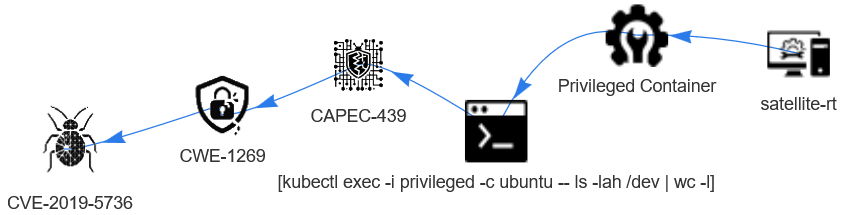
\includegraphics[width=0.8\textwidth]{attack-graph}
    \caption{Visualisierung eines Angriffspfads}
    \label{fig:attack-graph}
\end{figure}

\par Ein Teil der Informationen stammt direkt aus dem Angriffstool und wird aus der Datenbank gelesen. Dazu gehört zum einen der Gerätename, auf dem das \gls{at} ausgeführt wird. Wenn ein Angriff über die \gls{cli} eines Tools ausgeführt wird, ist der Name dieses Tools in der Datenbank hinterlegt, sowie das Kommando, dass die Ausführung des Angriffes startet. Diese Informationen müssen nicht zwangweise hinterlegt sein, sind aber in den meisten Fällen vorhanden. Über den Wert das Feldes \verb|tool_name| kann in der Übersicht aller Artefakte gefiltert werden.
\par Ein anderer Teil wird aus den \gls{acema} Daten zugeordnet. Alle relevanten Daten werden, wie in Listing \ref{list:go-embed} gezeigt, in der Funktion \verb|InitACEMA()|in eine Liste von Objekten vom Typ \verb|ACEMA_DATA| geladen. Wenn dem Artefakt über die Datenbank eine \gls{mitre}-Technik zugeordnet wurde, werden diese Daten nach dieser \verb|technique_id| durchsucht und bei dem \textit{ersten Match} \gls{capec} und \gls{cwe} zugeordnet. Diese Logik ist in der Funktion \verb|AddACEMA()| zu finden. Im \gls{acema}-Datensatz, der aktuell im Dashboard verwendet wird, ist es in weniger als 15\% der Fälle so, dass mehrere \glspl{capec} zu einer \gls{mitre}Technik gefunden werden. Häufiger (vgl. Schätzung aus Kapitel \ref{sec:impl-anwendungVonAcema}) kommt es vor, dass einem \gls{capec} mehrere \glspl{cwe} zugeordnet sind. Da nach dem Prinzip \textit{erster Match} die Daten für die Angriffspfadvisualisierung gesucht werden, ist diese Zuordnung mit Vorsicht zu genießen. Insbesonderes ist es wichtig dabei zu beachten ist, dass keine spezifischen \glspl{cve} zugeordnet werden, da hier die Fehlerrate über den \textit{ersten Match} noch größere wäre. Über \gls{acema} wird eine generelle Menge an möglichen \glspl{cve} gefunden, welcher spezifische \gls{cve} letztendlich von dem jeweiligen Tool ausgenutzt wird, kann darüber nicht klar zugeordnet werden. Um eine genaue Zuordnung herzustellen, ist ein manueller Eintrag vom \gls{at} in das Feld \verb|cve| des jeweiligen Artefakts nötig. Für die Daten \gls{capec} und \gls{cwe} wird dieses Risiko der möglicherweise ungenauen Zuordnung eingegangen, da es sich nicht um hochkritische Daten handelt. Zwischen \glspl{capec} und \glspl{cwe} die einer \gls{mitre}-Technik zugeordnet sind, ist immer eine deutliche Ähnlichkeit zu erkennen.
\par Für die textbasierte Erstellung von Diagrammen wird in wissenschaftlichen Kreis oft die quell-offene Software \textit{GraphViz} und ihre standardisierte \gls{dot} Skriptsprache verwendet. Mithilfe dieser Tools ist es möglich, auf eine flexible und klare Weise  Diagramme textuell zu definieren und in wissenschaftliche Arbeitsschritte zu integrieren \autocite{Graphviz,DOTLanguage}. Im Dashboard wurde die Erstellung von Graphen im \gls{dot} Format genutzt, da sich ein einfacher Graph innerhalb weniger Zeilen ausdrücken lässt und es \gls{js} Pakete gibt, die die Umwandlung von Text zu Graph komfortabel zulassen.
\par Die Erstellung eines \gls{dot}-Graphen in \gls{html} erfolgt in mehreren Schritten, um eine dynamische und visuelle Darstellung zu ermöglichen. Voraussetzung ist, dass die zu visualisierenden Daten des Artefakts in der Datenbank existieren. Außerdem ist die Vorlage des Graphen als ein Go String definiert. Diese Vorlage dient als Grundgerüst für den Graphen und enthält Platzhalter, die später durch spezifische Daten gefüllt werden. Die Struktur des Templates ist so gestaltet, dass sie die grundlegenden Elemente eines \gls{dot}-Graphen, wie Knoten, Kanten und Attribute, klar definiert. In Abbildung \ref{fig:vis-graph-steps} ist der Prozess visuell dargestellt. Der Fluss der Daten ist dort mit Pfeilen dargestellt, die Blöcke beschreiben die durchgeführten Aktionen in der jeweiligen Umgebung.
\par Der Prozess beginnt mit dem Auslesen der Daten aus der Datenbank, sobald die Detailseite eines Artefakts aufgerufen wird. Bei jedem Aufruf der Seite wird der Graph neu erstellt, um auf aktualisierte Daten reagieren zu können. Die Artefaktdaten existieren jetzt als ein Objekt in Go und können zum dynamischen Füllen der Lücken im \gls{dot}-Template genutzt weden. Dadurch entsteht ein individuell angepasster \gls{dot}-Graph, der die spezifischen Daten widerspiegelt.
\par Der dritte Schritt umfasst die Übergabe der gefüllten Daten an das Go-Template \verb|artifacts/show.tmpl|. Die Übergabe der Daten erfolgt mithilfe des Web-Frameworks \textit{Gin}. Dieses Go-Template ist für die Generierung des finalen \gls{html}-Codes zuständig, der den \gls{dot}-Graph enthält \autocite{GingonicGinGin}.
\par Anschließend werden im vierten Schritt die Daten aus den übergebenen Variablen gelesen und in die für \textit{Hotwire Stimulus} benötigten Felder eingefügt, um sie später in \gls{js} weiterverarbeiten zu können. Die Daten werden dabei als Werte in \gls{html}-Attributen gesetzt und sind nicht direkt für den Nutzer sichtbar. \textit{Stimulus} benötigt hierbei Daten im Attribut \verb|data-xxx-value|. Dieses Attribut enthält den \gls{dot}-String. Außerdem wird in \verb|data-xxx-target| der Name des \gls{html}-Elements definiert, der als Zielcontainer für die Visualisierung des Graphen dient. Der \gls{js}-Controller von Hotwire sorgt dafür, dass die Daten dynamisch an das Zielelement übergeben werden, wodurch die Interaktivität der Darstellung gewährleistet wird \autocite{StimulusReference}.
\par Im letzten Schritt übernimmt der \gls{js}-Controller, in diesem Fall vis\_controller.js, die Verantwortung. Dieser liest den dynamisch generierten \gls{dot}-String aus dem \gls{html}-Attribut aus und verarbeitet sie mit der Funktion \verb|parseDOTNetwork| aus dem \gls{js}-Paket vis-network weiter. Dieses Paket wandelt den \gls{dot}-Quellcode in eine visuelle Graphenstruktur um, die anschließend in das Zielelement gerendert wird. Durch die Verwendung von vis-network wird eine Darstellung gewährleistet, die es dem Nutzer erlaubt mit dem Graphen zu interagieren \autocite{VisjsVisnetwork2024}. Detailierte Informationen zu den Funktionen des Graphen wurden in Kapitel \ref{sec:auswahlDerVisualisierungstechniken} gegeben.
\par Insgesamt bietet dieser Prozess eine effiziente Methode, um \gls{dot}-Quellcode dynamisch zu erstellen, in \gls{js} zu interaktiven Graphen zu verarbeiten und in \gls{html} visuell darzustellen.

\begin{figure}
    \centering
    \begin{tikzpicture}[node distance=2cm, auto]

        % Nodes
        \node (start) [rectangle, draw, text centered] {Daten existieren in Datenbank};
        \node (process1) [rectangle, draw,below of=start] {Dynamisches Füllen der Lücken im \gls{dot}-Template};
        \node (process2) [rectangle, draw,below of=process1] {Setzen von \textit{Hotwire Stimulus} \verb|value| und \verb|target|};
        \node (process3) [rectangle, draw,below of=process2] {\textit{\gls{html}} ist Transfermedium der Daten};
        \node (process4) [rectangle, draw,below of=process3] {Verarbeitung von \gls{dot} zu \textit{Vis Network}};
        \node (stop) [rectangle, draw,below of=process4] {Visualisierung des Graphen};

        % Arrows
        \draw [->, thick] (start) -- (process1) node[midway, left] {Schritt 1: \textit{Datenbank} nach Go};
        \draw [->, thick] (process1) -- (process2) node[midway, right] {Schritt 2: Go nach \textit{Go Template}};
        \draw [->, thick] (process2) -- (process3) node[midway, left] {Schritt 3: \textit{Go Template} nach \textit{\gls{html}-Attribut}};
        \draw [->, thick] (process3) -- (process4) node[midway, right] {Schritt 4: \textit{\gls{html}-Attribut} nach \textit{\gls{js}}};
        \draw [->, thick] (process4) -- (stop) node[midway, left] {Schritt 5: \textit{\gls{js}} nach \textit{\gls{html}-Element}};

    \end{tikzpicture}
    \caption{Schritte zur Erstellung des Graphen}
    \label{fig:vis-graph-steps}
\end{figure}

\section{Sonstige Implementierungen}
\label{sec:impl-others}
Neben den bereits genannten Themen, wurden viele weitere kleinere Änderungen am Dashboard vorgenommen, um die Funktionalität und die Benutzererfahrung zu verbessern. Auf eine Auswahl dieser sonstigen Verbesserungen wird in diesem Kapitel eingegangen.
\subsection{Weiterführende Informationen zu Techniken}
\par Wie in Kapitel \ref{sec:datenquellen} beschrieben, bieten sich drei wissenschaftliche Konstrukte an, aus denen Techniken in die Matrix im Dashboard übernommen werden können. Bis auf zwei Techniken können alle im Dashboard angezeigten Techniken mindestens zwei Techniken aus \gls{tm4k}, \gls{mitre} \gls{attack} Matrix oder dem \gls{wg11} Report zugeordnet werden. Wie in \ref{sec:impl-anwendungVonAcema} beschrieben, wurde diese Zuweisung über einen Vergleich der Beschreibungen der jeweiligen Techniken manuell vorgenommen.
Um diese Zuweisungen nicht nur ohne weitere Funktion textuell darzustellen, wurde eine Verlinkung zu weiterführenden Informationen auf den Seiten \autocite{MITREATTCK} und \autocite{TacticsThreatMatrix} hinzugefügt. Eine Onlinequelle zu den O-RAN Bedrohungen gibt es bisher nicht, diese sind alleine in einem Microsoft Word Dokument veröffentlicht. Die URL, an die nach einem Klick weitergeleitet wird, ist dynamisch aus den Daten der Technik zusammengesetzt. Für die \gls{mitre} \gls{attack} Webseite setzt sich die URL so zusammen: \par \verb|attack.mitre.org/techniques/{Technik-ID}/{Subtechnik-ID}|
\par Microsofts \gls{tm4k} Seite nutzt für die URLs nicht die eindeutige ID, sondern den Titel der Technik. Die URL kann also wie folgt definiert werden: \par \verb|microsoft.github.io/[...]/techniques/{Technik-Titel}|
\par Die Zuordnung zu den Quellen wird auch farblich gekennzeichnet. Wenn kein Wert angezeigt wird, ist keine weitere Zuordnung möglich.
\subsection{Verbesserung der Zeitleiste}
Die Zeitleiste ist ein wichtiges Feature im Dashboard. Es zeigt visuell aufbereitet, in welchem Zeitraum ein Angriff ausgeführt wurde. Es bringt jedoch einige technische Herausforderungen mit sich, für die im Folgenden eine Lösung präsentiert wird.
\par Ein Angriff dauert in der Regel nur wenige Sekunden, eine Darstellung auf einer Zeitleiste die mehrere Stunden oder Tage umfasst ist daher schwierig. Das \gls{js} Framework \textit{Apexcharts.js}, welches für die Visualisierung der Zeitleisten verwendet wird, bietet eine Funktion die es erlaubt, auch kleinste zeitliche Abschnitte in einem großen Zeitraum zu erkennen. Die Funktion fügt zum Start- und Endzeitpunkt eines Angriffs jeweils einen Punkt hinzu, dessen Größe nicht mit der Dauer des Angriffs skaliert. In einer Übersicht über mehrere Stunden oder Tage ist jedes Artefakt mit einem gleichgroßen Punkt gekennzeichnet. Eine detailierte Ansicht kann dann über die Zoomfunktion erreicht werden. Dabei kann direkt in der Zeitliste durch \textit{Klicken-und-Ziehen} der Maus eine Zeitspanne ausgewählt werden. Diese beiden Funktionen werden über die Konfiguration in der Datei \verb|assets\js\controllers\timeline_controller.js| aktiviert.
\par Bei der Darstellung von einer großen Menge von Artefakten auf der Zeitleiste ist eine deutliche Einbuse der Performance zu spüren. Über subjektives Empfinden wurde eine Grenze von 100 Artefakten gefunden, bis zu der die Visualisierung ohne merkliche Verzögerung möglich ist. Die Begrenzung wird im Logik Teil der Anwendung angewendet, bevor die Daten überhaupt vom Server in die \gls{html} Datei eingebettet werden. Die Datenbankabfrage sortiert die Daten absteigend nach Startdatum, es werden daher die 100 Artefakte angezeigt, die die Daten der zuletzt ausgeführten Angriffe enthalten \autocite{$sortAggregationMongoDB}. Der dazugehörige Quellcode ist in Listing \ref{list:go-sort} dargestellt.
\begin{code}[caption=Sortierung der Datenbankobjekte, label={list:go-sort}]
    options.Find().SetSort(bson.D{{Key: "timestamp_start", Value: -1}})
\end{code}

\subsection{Vereinfachung der Datenstruktur eines Artefakts}
Über den Zeitraum der Implementierung haben sich nicht wenige Änderungen in der Datenstruktur eines Artefakts ergeben. In einer NoSQL Datenbank muss prinzipiell keine feste Struktur vorhanden sein, ist jedoch für das Auslesen eines Objekts in die definierte Datenstruktur in Go nötig. Da die Serialisierung von Python zu JSON in einer anderen Anwendung und von anderen Personen implementiert wurde als die Deserialisierung von JSON zu Go, war eine Absprache von großer Wichtigkeit. So wurde aus dem Feld \verb|mitre| mit Datentyp \verb|String| zuerst eine Liste um auch eine Zuordnung zu mehreren \gls{mitre} Techniken abbilden zu können. Später wurden alle Informationen über Techniken und Taktik in ein Feld vereint. Das Feld \verb|command| wurde angepasst, um die Ausführung mehrerer Kommandos während eines Angriffs modellieren zu können. Weitere kleinere Änderungen führten zu dem Schema, welches im Anhang \ref{app:db-schema} dargestellt ist. Eine Erweitung dieses Schemas ist einfach möglich. Das hinzugekommene Feld muss dafür in der Datei \verb|pkg\artifacts\model.go| in der \verb|struct| Definition eines Artefakts hinzugefügt werden, wie in Listing \ref{list:new-field} demonstriert ist.
\begin{code}[caption=Hinzufügen eines Feldes zum Schema in Go, label={list:new-field}]
    type Artifact struct {
            ID          primitive.ObjectID  `bson:"_id" json:"id"`
            IP          string              `bson:"ip" json:"ip"`
            ...
            NewField    float64             `bson:"new_field" json:"new_field"`
        }
\end{code}

\subsection{Verknüpfung zwischen Kampagnen und Artefakten}
Kampagnen sind ein Bestandteil des \gls{at} die es ermöglichen mehrere Angriffe zu einer übergeordneten Einheit zusammenzufassen. In der Datenbank sind Kampagnen und Artefakte über eine \textit{One-to-Many} Relation implementiert. Bisher war es im Dashboard nicht möglich die Artefakte aufzulisten, die einer Kampagne zugeordnet sind. Über eine einzelne Datenbankabfrage können die Artefakte gefunden werden, die einer Kampagne zugeordnet sind. Diese werden jetzt auf der Detailsseite einer Kamapgne angezeigt. Außerdem wurde eine Zeitleiste hinzugefügt, die diese Artefakte im Zeitraum der Laufzeit der Kamapagne anzeigt. Dafür wurde die bestehende Logik der Artefaktzeitleiste auf der Übersichtseite aller Artefakte wiederverwendet. Das Ergebnis ist in Abbildung \ref{fig:campaign} dargestellt. Diese Funktion setzt die übergreifende Anforderung um, alle relevanten Daten auch über das Dashboard abrufen zu können, ohne auf die Datenbank direkt mithilfe der MongoDB Query Language oder anderer externer Tools zugreifen zu müssen.

\begin{figure}
    \centering
    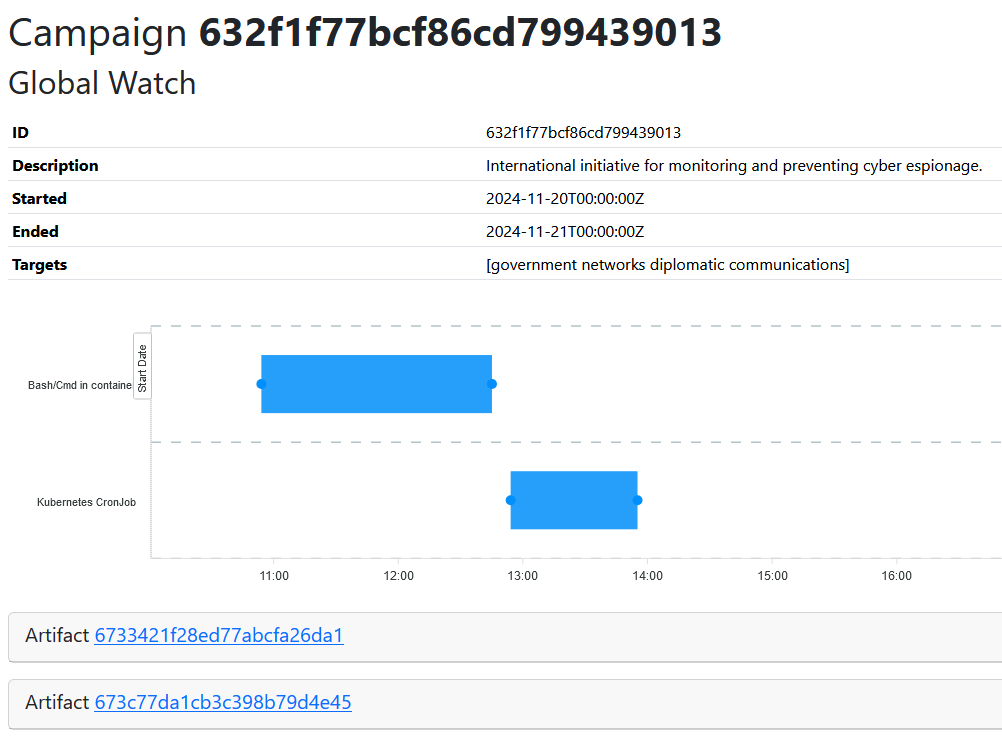
\includegraphics[width=0.6\textwidth]{campaign.png}
    \caption{Zuordung von Artefakten zu einer Kampagne und Visualierung der Artefakte auf einer Zeitleise.}
    \label{fig:campaign}
\end{figure}
\chapter{Diskussion}
\label{chap:diskussion}
\section{Interpretation der Ergebnisse}
\todo{Hier nochmal den Inhalt überdenken.}
Erfolg der Implementierung:
Was hat gut funktioniert? Wo gab es unerwartete Herausforderungen?

Einsatz in der Praxis:
Inwiefern ist das Ergebnis in der Praxis anwendbar? Welche Verbesserungen sind nötig?

Vergleich mit bestehenden Lösungen:
Falls bekannt, könnten Sie Ihre Lösung mit anderen Ansätzen vergleichen.

\section{Limitation}
\label{sec:limitationen}
Die Analyse und Implementierung unterliegt spezifischen Einschränkungen, die sowohl durch methodische als auch durch technologische Faktoren bedingt sind. Dabei sind insbesondere die Generalisierbarkeit der Ergebnisse und die Abdeckung aller relevanten Daten kritisch zu betrachten. \todo{Über "Generalisierbarkeit der Ergebnisse und die Abdeckung aller relevanten Daten" noch schreiben oder hier streichen.} Weiterhin beeinflussen die Auswahl und die Qualität der genutzten Datenquellen sowie deren Aktualität die Aussagekraft der Analyse. \todo{Diesen Absatz nochmal betrachten.}
\subsection{Generelle Limitationen}
\label{limitation-generell}
\par Die \gls{nvd} gilt als zentrale Resource für Informationen über öffentlich bekannte Sicherheitslücken. Daher scheint es auch als verlässliche Quelle für die IT-Sicherheitsbranche und Forschungszwecke. Laut einer Veröffentlichung vom 13. Februar 2024 kommt das \gls{nist} nicht der Abarbeitung der eingereichten \glspl{cve} hinterher und arbeitet daran, die Verzögerung bei der Analyse zu beheben \autocite{NVDProgramAnnouncement}. Am 13. November 2024 kündigte das \gls{nist} an, alle neu eingereichten \gls{cve} direkt verarbeiten zu können. Die Abarbeitung der zurückgestellten Daten dauert weiterhin an. Die Daten aus der \gls{nvd} sind daher aktuell  nicht auf dem neusten Stand \autocite{NationalVulnerabilityDatabase2024}. Eine vom \textit{IT Security Infrastructures Lab} der \textit{Friedrich-Alexander Universität Erlangen-Nürnberg} veröffentliche Studie vom \citedate{wunderNVDUsersAttitudes2024} unterlegt diese Feststellung mit empirischen Daten. Demnach sind fast 40\% der Befragten jährlich, monatlich, wöchentlich oder täglich von der verzögerten Veröffentlichung von neuen \glspl{cve} betroffen \autocite{wunderNVDUsersAttitudes2024}. Die damit zusammenhängenden und weitere technische Schwierigkeiten beeinflussen auch die Abfrageverfügbarkeit und Abfragegeschwindigkeit von Daten aus der \gls{nvd}. Für \gls{acema} haben die Einschränkungen weitreichende Konsequenzen, von verlangsamter Abfragegeschwindigkeit des \gls{cvss} für \glspl{cve} bis hin zur vollständigen Abwesenheit von \gls{cvss} Daten, die eine integrale Rolle für die Datenanalyse spielen.
%
\subsection{Limitation von ACEMA}
\label{limitationen-acema}
Die Implementierung von \gls{acema} nutzt für die Bewertung das \gls{cvss} in Version \textit{v2.0} aus dem Jahr 2007 \autocite{Acema_oranOCloud_Data_GatheringpyMaster}. Seit dem 27. Juni 2024 unterstützt die \gls{nvd} das Bereitstellen von Daten in \textit{v4.0} des \gls{cvss} \autocite{NVDCVSSV40}. Nicht nur ist die in \gls{acema} genutzte Version durch zwei \textit{major}-Versionen überholt, seit dem 13. Juli 2022 werden in der Datenbank keine neuen Angriffsvektordaten, qualitative Schweregrad-Bewertungen oder Schweregrad-Werte in \gls{cvss} \textit{v2.0} erstellt \autocite{RetirementCVSSV2}. Der Fall von unvollständigen Daten ist in der Bearbeitung dieses Projekts nicht vorgekommen, da alle im Ergebnisse des Mappings aufgeführten \glspl{cve} im Jahr 2021 oder früher veröffentlicht wurden. Es ist jedoch theoretisch möglich, dass diese Einschränkung bei der weiteren Nutzung dieser Methode zu fehlenden Daten führen kann.
%
\par Das von \gls{acema}, mithilfe des \gls{cti} Repositories, erstellte Mapping von \gls{mitre}-Technik zu \gls{capec} (Schritt 1 in Abbildung \ref{fig:mitre_mapping}) findet nicht alle \gls{capec}. Die Dokumentation im Repository erklärt zu dem Finden von \glspl{capec}: \gls{capec} IDs können dort für die Techniken gefunden werden, wo das unter externen Referenzen das Attribut \textit{source\_name} den Wert \verb|capec| hat \autocite{CtiUSAGEmdMaster} \autocite{CtiUSAGECAPECmdMaster}. \citeauthor{klementSecuring6GTransition2024} nutzen in ihrer Implementierung die Daten aus dem \textit{enterprise-attack/attack-pattern} Teil des Repositories \autocite{klement2023acema}. Nach demselben Prinzip kann auch der \textit{capec/2.1/attack-pattern} Teil des Repositories durchsucht werden. Der Unterschied in den beiden Datensätzen liegt darin, was der Hauptzweck der Daten ist. Der \textit{enterprise-attack} Teil enthält die Datenstruktur \todo{anderes Wort für Datenstruktur} der \gls{mitre} \gls{attack} \textit{Enterprise}-Matrix, mit Daten wie der \gls{mitre}-Technik ID, Taktik und angreifbare Platform sowie manchmal Referenzen zu \gls{mitre}-Techniken. Der \gls{capec} Teil enthält die Datenstruktur \todo{anderes Wort für Datenstruktur} des \gls{capec}-Frameworks, mit Daten wie \gls{capec} ID, Konsequenzen und Voraussetzungen für die Ausnutzung sowie manchmal Referenzen zu \gls{mitre}-Techniken. Es zeigt sich in den Daten aus Tabelle \ref{tab:comparison_with_diff}, dass über den \textit{\gls{capec}} Teil eine vollständigere Abbildung von \gls{mitre}-Technik zu \gls{capec} ID möglich ist. Die beiden Implementierungen des Mappings wurden auf demselben Datensatz aus Anhang \ref{app:mapping-dataset} ausgeführt, der ein direkter Export der Daten aus der Dashboardmatrix ist.
%

\begin{table}[H]
    \centering
    \caption{Vergleich der Daten zwischen eigener Implementierung und ACEMA Implementierung}
    \begin{tabular}{|l|c|c|c|}
        \hline
        \textbf{Metrik}     & \textbf{Eigene Impl.} & \textbf{ACEMA Impl.} & \textbf{Differenz (\%)} \\
        \hline
        Techniken           & 27                    & 27                   & 0 \%                    \\
        \hline
        Techniken mit CAPEC & 14                    & 3                    & -75 \%                  \\
        \hline
        Einzigartige CAPECs & 25                    & 6                    & -76 \%                  \\
        \hline
        Einzigartige CWEs   & 39                    & 15                   & -62 \%                  \\
        \hline
    \end{tabular}
    \label{tab:comparison_with_diff}
\end{table}

\section{Ausblick}
\label{sec:ausblick}
Starten von \gls{acema} aus dem Dashboard heraus, dafür entweder \gls{acema} in GoLang implementieren oder python Wrapper oä\dots \\
Live-Updates im Dashboard, wenn neue Artefakte eingefügt oder Kampagnen starten. \\
Mapping von Technik zu CVE auch für MS-Techniken implementieren. \\
Aus \gls{acema}: Manuelle Zuordnung unterstützen durch maschinelles Lernen. \\


\chapter{Zusammenfassung}
\label{chap:zusammenfassung}
\section{Zusammenfassung}
\label{sec:zusammenfassung}
\section{Ausblick}
\label{sec:ausblick}
%
\printbibliography
%
\appendix
\addchap{Anhang}
\chapter{Quellcodes zur Arbeit}
\label{app:sourcecode}
In der Arbeit werden verschiedene Quellcodes referenziert. Es folgt eine Auflisting der Quellcodes, die in der Arbeit verwendet wurden, und wo sie zu finden sind.
\begin{itemize}
    \item \textbf{Quellcode des Dashboards}: Der Quellcode des Dashboards ist in einem Git-Repository auf GitLab verfügbar. Dieselbe Gitlab-Instanz enthält auch die Projekte und Quellcodes für andere Komponenten des Forschungsprojekts. Zum aktuellen Zeitpunkt ist der Zugriff auf das Repository nur für autorisierte Personen möglich. Das Forschungsprojekt verfolgt das Ziel, alle Quellcodes nach Abschluss des Projekts zu veröffentlichen, voraussichtlich im ersten Halbjahr des Jahres 2025. Der genaue Link zum Repository wird zu gegebener Zeit unter \url{https://www.5g-foran.com/} veröffentlicht.
    \item \textbf{Quellcode von \citeauthor{klementSecuring6GTransition2024}}: Der Quellcode der Implementation von \citeauthor{klementSecuring6GTransition2024} ist in einem Git-Repository auf GitHub verfügbar. Im Fließtext dieser Arbeit wird dieser Quelltext als \textit{originaler Quellcode} bezeichnet. Der Quellcode ist unter folgendem Link verfügbar: \url{https://github.com/fklement/acema_oran}
    \item \textbf{Fork des Quellcode von \citeauthor{klementSecuring6GTransition2024}}: Der Quellcode des Forks von \citeauthor{klementSecuring6GTransition2024} ist in einem Git-Repository auf GitHub verfügbar. Der Fork enthält die eigens vorgenommenen Änderungen und wird im Fließtext dieser Arbeit als \textit{verbesserter Quellcode} bezeichnet. Der Quellcode ist unter folgendem Link verfügbar: \url{https://github.com/dumpeldown/acema_oran}
\end{itemize}

\label{app:attack-szenarien}
\todo{Daten aus https://procyde.atlassian.net/wiki/spaces/FORAN/pages/662634527/Angriffsszenarien+bersicht}

\chapter{Beispiel ACEMA JSON Output}
\label{app:acema-output}
\begin{code}
{
 "scan_date": "2023-08-22",
 "scan_runtime": "00h 16m and 41.62s",
 "data": [
  {
   "technique_id": "T1498",
   "t_findings": []
  },
  {
   "technique_id": "T1068",
   "t_findings": [
    {
     "capec_id": "CAPEC-69",
     "c_findings": [
      {
       "cwe": "CWE-250",
       "cves": [
        {
         "id": "CVE-2007-4217",
         "score": [
          "V2",
          7.2,
          "HIGH"
         ],
         "v2_score": 7.2,
         "v2_exploitability_score": 3.9,
         "v2_impact_score": 10.0,
         "v2_vector": "AV:L/AC:L/Au:N/C:C/I:C/A:C",
         "access_vector": "LOCAL",
         "full_metrics": [
          {
           "source": "nvd@nist.gov",
           "type": "Primary",
           "cvssData": {
            "version": "2.0",
            "vectorString": "AV:L/AC:L/Au:N/C:C/I:C/A:C",
            "accessVector": "LOCAL",
            "accessComplexity": "LOW",
            "authentication": "NONE",
            "confidentialityImpact": "COMPLETE",
            "integrityImpact": "COMPLETE",
            "availabilityImpact": "COMPLETE",
            "baseScore": 7.2
           },
           "baseSeverity": "HIGH",
           "exploitabilityScore": 3.9,
           "impactScore": 10.0,
           "acInsufInfo": false,
           "obtainAllPrivilege": true,
           "obtainUserPrivilege": false,
           "obtainOtherPrivilege": false,
           "userInteractionRequired": false
          }
         ],
         "description": "Stack-based buffer overflow in the domacro function in ftp in IBM AIX 5.2 and 5.3 allows local users to gain privileges via a long parameter to a macro, as demonstrated by executing a macro via the '$' command.",
         "cpe_vulnerable": true,
         "cpe_criteria": "cpe:2.3:o:ibm:aix:5.2:*:*:*:*:*:*:*",
         "published": "2007-11-05T16:46:00.000",
         "last_modified": "2017-07-29T01:32:47.160"
        }
       ],
       "cwe_info": {
        "cwe_id": "250",
        "name": "Execution with Unnecessary Privileges",
        "weakness_abstraction": "Base",
        "status": "Draft",
        "description": "The software performs an operation at a privilege level that is higher than the minimum level required, which creates new weaknesses or amplifies the consequences of other weaknesses.",
        "extended_description": "New weaknesses can be exposed because running with extra privileges, such as root or Administrator, can disable the normal security checks being performed by the operating system or surrounding environment. Other pre-existing weaknesses can turn into security vulnerabilities if they occur while operating at raised privileges. Privilege management functions can behave in some less-than-obvious ways, and they have different quirks on different platforms. These inconsistencies are particularly pronounced if you are transitioning from one non-root user to another. Signal [...]
        "related_weaknesses": "::NATURE:ChildOf:CWE ID:657:VIEW ID:1000:ORDINAL:Primary::NATURE:ChildOf:CWE ID:269:VIEW ID:1000::",
        "weakness_ordinalities": "",
        "applicable_platforms": "::LANGUAGE CLASS:Language-Independent:LANGUAGE PREVALENCE:Undetermined::TECHNOLOGY CLASS:Mobile:TECHNOLOGY PREVALENCE:Undetermined::",
        "background_details": "",
        "alternate_terms": "",
        "modes_of_introduction": "::PHASE:Implementation:NOTE:REALIZATION: This weakness is caused during implementation of an architectural security tactic.::PHASE:Installation::PHASE:Architecture and Design:NOTE:If an application has this design problem, then it can be easier for the developer to make implementation-related errors such as CWE-271 (Privilege Dropping / Lowering Errors). In addition, the consequences of Privilege Chaining (CWE-268) can become more severe.::PHASE:Operation::",
        "exploitation_factors": "",
        "likelihood_of_exploit": "",
        "common_consequences": "::SCOPE:Confidentiality:SCOPE:Integrity:SCOPE:Availability:SCOPE:Access Control:IMPACT:Gain Privileges or Assume Identity:IMPACT:Execute Unauthorized Code or Commands:IMPACT:Read Application Data:IMPACT:DoS: Crash, Exit, or Restart:NOTE:An attacker will be able to gain access to any resources that are allowed by the extra privileges. Common results include executing code, disabling services, and reading restricted data.::",
        "detection_methods": "::METHOD:Manual Analysis:DESCRIPTION:This weakness can be detected using tools and techniques that require manual (human) analysis, such as penetration testing, threat modeling, and interactive tools that allow the tester to record and modify an active session.::METHOD:Black Box:DESCRIPTION:Use monitoring tools that examine the software's process as it interacts with the operating system and the network. This technique is useful in cases when source code is unavailable, if the software was not developed by you, or if you want to verify that the build phase did not [...]
        "potential_mitigations": "::PHASE:Architecture and Design Operation:STRATEGY:Environment Hardening:DESCRIPTION:Run your code using the lowest privileges that are required to accomplish the necessary tasks [REF-76]. If possible, create isolated accounts with limited privileges that are only used for a single task. That way, a successful attack will not immediately give the attacker access to the rest of the software or its environment. For example, database applications rarely need to run as the database administrator, especially in day-to-day operations.::PHASE:Architecture and Design[...]
        "observed_examples": "::REFERENCE:CVE-2007-4217:DESCRIPTION:FTP client program on a certain OS runs with setuid privileges and has a buffer overflow. Most clients do not need extra privileges, so an overflow is not a vulnerability for those clients.:LINK:[shortened] runs with privileges and calls another program with the same privileges, which allows read of arbitrary files.:LINK:[shortened] incorrectly [...]
        "functional_areas": "",
        "affected_resources": "",
        "taxonomy_mappings": "::TAXONOMY NAME:7 Pernicious Kingdoms:ENTRY NAME:Often Misused: Privilege Management::TAXONOMY NAME:The CERT Oracle Secure Coding Standard for Java (2011):ENTRY ID:SER09-J:ENTRY NAME:Minimize privileges before deserializing from a privilege context::",
        "related_attack_patterns": "::104::470::69::",
        "notes": "::TYPE:Relationship:NOTE:There is a close association with CWE-653 (Insufficient Separation of Privileges). CWE-653 is about providing separate components for each privilege; CWE-250 is about ensuring that each component has the least amount of privileges possible.::TYPE:Maintenance:NOTE:CWE-271, CWE-272, and CWE-250 are all closely related and possibly overlapping. CWE-271 is probably better suited as a category. Both CWE-272 and CWE-250 are in active use by the community. The least privilege phrase has multiple interpretations.::"
       }
      },
      {
       "cwe": "CWE-15",
       "cves": [],
       "cwe_info": {
        "cwe_id": "15",
        "name": "External Control of System or Configuration Setting",
        "weakness_abstraction": "Base",
        "status": "Incomplete",
        "description": "One or more system settings or configuration elements can be externally controlled by a user.",
        "extended_description": "Allowing external control of system settings can disrupt service or cause an application to behave in unexpected, and potentially malicious ways.",
        "related_weaknesses": "::NATURE:ChildOf:CWE ID:642:VIEW ID:1000:ORDINAL:Primary::NATURE:ChildOf:CWE ID:610:VIEW ID:1000::NATURE:ChildOf:CWE ID:20:VIEW ID:700:ORDINAL:Primary::",
        "weakness_ordinalities": "",
        "applicable_platforms": "",
        "background_details": "",
        "alternate_terms": "",
        "modes_of_introduction": "::PHASE:Implementation:NOTE:Setting manipulation vulnerabilities occur when an attacker can control values that govern the behavior of the system, manage specific resources, or in some way affect the functionality of the application.::PHASE:Implementation:NOTE:REALIZATION: This weakness is caused during implementation of an architectural security tactic.::",
        "exploitation_factors": "",
        "likelihood_of_exploit": "",
        "common_consequences": "::SCOPE:Other:IMPACT:Varies by Context::",
        "detection_methods": "",
        "potential_mitigations": "::PHASE:Architecture and Design:STRATEGY:Separation of Privilege:DESCRIPTION:Compartmentalize the system to have safe areas where trust boundaries can be unambiguously drawn. Do not allow sensitive data to go outside of the trust boundary and always be careful when interfacing with a compartment outside of the safe area. Ensure that appropriate compartmentalization is built into the system design, and the compartmentalization allows for and reinforces privilege separation functionality. Architects and designers should rely on the principle of least privilege [...]
        "observed_examples": "",
        "functional_areas": "",
        "affected_resources": "",
        "taxonomy_mappings": "::TAXONOMY NAME:7 Pernicious Kingdoms:ENTRY NAME:Setting Manipulation::TAXONOMY NAME:Software Fault Patterns:ENTRY ID:SFP25:ENTRY NAME:Tainted input to variable::",
        "related_attack_patterns": "::13::146::176::203::270::271::69::76::77::",
        "notes": ""
       }
      }
     ]
    }
   ]
  }
 ]
}   
\end{code}
\chapter{Mapping Datensatz}
\label{app:mapping-dataset}
\begin{table}[!ht]
    \caption{Mapping von Threat ID zu MITRE-Technik und MITRE-Taktik}
    \centering
    \begin{longtable}{|l|l|l|l|l|}
    \hline
        Name & Domain & Description & Technique & Tactic \\ \hline
        T-IMG-01 & enterprise-attack & Compromised image In registry & T1195.002 & TA0001 \\ \hline
        T-IMG-01 & enterprise-attack & Compromised image In registry & T1525 & TA0001 \\ \hline
        T-IMG-01 & enterprise-attack & Application vulnerability & T1190 & TA0001 \\ \hline
        T-GEN-02 & enterprise-attack & Exposed sensitive interfaces & T1133 & TA0001 \\ \hline
        T-GEN-02 & enterprise-attack & Exposed sensitive interfaces & T1078 & TA0007 \\ \hline
        T-GEN-02 & enterprise-attack & Exposed sensitive interfaces & T1609 & TA0001 \\ \hline
        T-GEN-02 & enterprise-attack & Exposed sensitive interfaces & T1059 & TA0007 \\ \hline
        T-ADMIN-02 & enterprise-attack & Exec into container & TT1204 & TA0002 \\ \hline
        T-O2-01 & enterprise-attack & Exec into container & T1610 & TA0002 \\ \hline
        T-VM-C-03 & enterprise-attack & Exec into container & T1612 & TA0002 \\ \hline
        T-VM-C-04 & enterprise-attack & Exec into container & T1543 & TA0002 \\ \hline
        T-VM-C-01 & enterprise-attack & Bash or cmd inside container & T1542 & TA0002 \\ \hline
        T-VM-C-01 & enterprise-attack & Bash or cmd inside container & T1611 & TA0002 \\ \hline
        T-ADMIN-02 & enterprise-attack & Bash or cmd inside container & T1053.007 & TA0002 \\ \hline
        T-ADMIN-02 & enterprise-attack & Bash or cmd inside container & T1528 & TA0002 \\ \hline
        T-HW-01 & enterprise-attack & Bash or cmd inside container & T1070 & TA0002 \\ \hline
        T-HW-01 & enterprise-attack & Bash or cmd inside container & T1036 & TA0002 \\ \hline
        T-IMG-01 & enterprise-attack & Bash or cmd inside container & T1036.005 & TA0002 \\ \hline
        T-IMG-01 & enterprise-attack & Bash or cmd inside container & T1552 & TA0002 \\ \hline
        T-IMG-01 & enterprise-attack & New container & T1613 & TA0002 \\ \hline
        T-IMG-01 & enterprise-attack & New container & T1046 & TA0002 \\ \hline
        T-IMG-04 & enterprise-attack & New container & T1210 & TA0002 \\ \hline
        T-IMG-04 & enterprise-attack & New container & T1530 & TA0002 \\ \hline
        T-GEN-01 & enterprise-attack & Application exploit (RCE) & T1485 & TA0002 \\ \hline
        T-VM-C-01 & enterprise-attack & Backdoor container & T1496 & TA0003 \\ \hline
        T-VM-C-01 & enterprise-attack & Backdoor container & T1498 & TA0003 \\ \hline
        T-VL-02 & enterprise-attack & Backdoor container & T1499 & TA0003 \\ \hline
        T-VL-02 & enterprise-attack & Backdoor container & TA0003 & ~ \\ \hline
        T-VM-C-02 & enterprise-attack & Writable hostPath mount & TA0003 & ~ \\ \hline
        T-VM-C-02 & enterprise-attack & Writable hostPath mount & TA0004 & ~ \\ \hline
        T-VM-C-02 & enterprise-attack & Writable hostPath mount & TA0008 & ~ \\ \hline
        T-VM-C-01 & enterprise-attack & Kubernetes CronJob & TA0003 & ~ \\ \hline
        T-GEN-02 & enterprise-attack & Container service account & TA0006 & ~ \\ \hline
        T-GEN-02 & enterprise-attack & Container service account & TA0008 & ~ \\ \hline
        T-GEN-02 & enterprise-attack & Container service account & TA0003 & ~ \\ \hline
        T-VM-C-01 & enterprise-attack & Privileged container & TA0004 & ~ \\ \hline
        T-VM-C-01 & enterprise-attack & Clear container logs & TA0005 & ~ \\ \hline
        T-O2-01 & enterprise-attack & Delete Kubernetes events & TA0005 & ~ \\ \hline
        T-VL-01 & enterprise-attack & Pod or container name similarity & TA0005 & ~ \\ \hline
        T-VL-01 & enterprise-attack & Pod or container name similarity & TA0005 & ~ \\ \hline
        T-IMG-01 & enterprise-attack & Pod or container name similarity & TA0005 & ~ \\ \hline
        T-IMG-01 & enterprise-attack & Pod or container name similarity & TA0005 & ~ \\ \hline
        T-IMG-03 & enterprise-attack & List Kubernetes secrets & TA0006 & ~ \\ \hline
        T-GEN-02 & enterprise-attack & Mount service principal & TA0006 & ~ \\ \hline
        T-ADMIN-02 & enterprise-attack & Application credentials in configuration files & TA0006 & ~ \\ \hline
        T-ADMIN-02 & enterprise-attack & Application credentials in configuration files & TA0008 & ~ \\ \hline
        T-VM-C-03 & enterprise-attack & Application credentials in configuration files & TA0006 & ~ \\ \hline
        T-VM-C-03 & enterprise-attack & Application credentials in configuration files & TA0008 & ~ \\ \hline
        T-GEN-02 & enterprise-attack & Access Managed Identity credentials & TA0006 & ~ \\ \hline
        T-O2-01 & enterprise-attack & Access Kubernetes API server & TA0007 & ~ \\ \hline
        T-O2-01 & enterprise-attack & Access Kubelet API & TA0007 & ~ \\ \hline
        T-O2-01 & enterprise-attack & Network mapping & TA0007 & ~ \\ \hline
        T-VM-C-03 & enterprise-attack & Instance Metadata API & TA0007 & ~ \\ \hline
        T-IMG-03 & enterprise-attack & Instance Metadata API & TA0007 & ~ \\ \hline
        T-VM-C-02 & enterprise-attack & Cluster internal networking & TA0008 & ~ \\ \hline
        T-IMG-01 & enterprise-attack & Images from a private registry & TA0009 & ~ \\ \hline
        T-IMG-04 & enterprise-attack & Images from a private registry & TA0009 & ~ \\ \hline
        T-VM-C-01 & enterprise-attack & Data destruction & TA0040 & ~ \\ \hline
        T-VM-C-04 & enterprise-attack & Resource hijacking & TA0040 & ~ \\ \hline
        T-VL-01 & enterprise-attack & Resource hijacking & TA0040 & ~ \\ \hline
        T-ADMIN-01 & enterprise-attack & Denial of service & TA0040 & ~ \\ \hline
        T-ADMIN-01 & enterprise-attack & Denial of service & TA0040 & ~ \\ \hline
        T-VM-C-04 & enterprise-attack & Denial of service & TA0040 & ~ \\ \hline
        T-VM-C-04 & enterprise-attack & Denial of service & TA0040 & ~ \\ \hline
        T-VM-C-05 & enterprise-attack & Denial of service & TA0040 & ~ \\ \hline
        T-VM-C-05 & enterprise-attack & Denial of service & TA0040 & ~ \\ \hline
    \end{longtable}
\end{table}

\chapter{Datenstruktur}
\label{app:db-schema}

\begin{figure}[H]
    \centering
    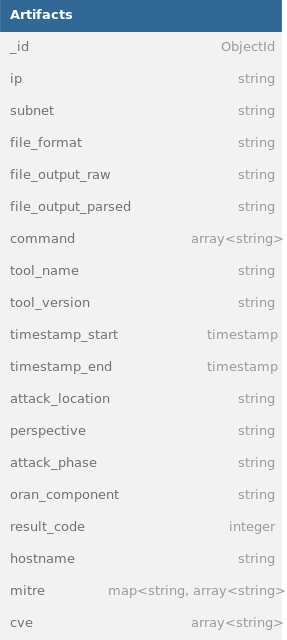
\includegraphics[width=0.5\textwidth]{db-schema}
    \caption{Struktur eines Artefakts in der Datenbank und in Go.}
\end{figure}




\KOMAoptions{open=any}
%
\chapter*{Erklärung}
%
Ich versichere, die von mir vorgelegte Arbeit selbstständig verfasst zu haben. Alle Stellen, die wörtlich oder sinngemäß aus veröffentlichten oder nicht veröffentlichten Arbeiten anderer oder der Verfasserin/des Verfassers selbst entnommen sind, habe ich als entnommen kenntlich gemacht. Sämtliche Quellen und Hilfsmittel, die ich für die Arbeit benutzt habe, sind angegeben. Im Rahmen der Arbeit habe ich ChatGPT als unterstützendes Werkzeug genutzt, insbesondere zur Erstellung von Visualisierungen in LaTeX. Alle generierten Inhalte wurden von mir überprüft, angepasst und auf die wissenschaftlichen Anforderungen meiner Arbeit abgestimmt.  Die Arbeit hat mit gleichem Inhalt bzw.\ in wesentlichen Teilen noch keiner anderen Prüfungsbehörde vorgelegen.
\\[3cm] \todo{Unterschrift einfügen!}
\begin{tabular}{@{}l@{}}%
\rule{0.35\textwidth}{0.4pt}\\
Ort, Datum%
\end{tabular}%
\hfill%
\begin{tabular}{@{}l@{}}%
\rule{0.45\textwidth}{0.4pt}\\
Unterschrift%
\end{tabular}%
%
%
\end{document}